%! program = pdflatex

\documentclass[12pt]{article}

%%% PACKAGES
\usepackage{ifpdf}
\usepackage{booktabs}   % for much better looking tables
\usepackage{array}      % for better arrays (eg matrices) in maths
\usepackage{paralist}   % very flexible & customisable lists (eg. enumerate/itemize, etc.)
%\usepackage{verbatim}   % adds environment for commenting out blocks of text & for better verbatim
\usepackage{subfigure}  % make it possible to include more than one captioned figure/table in a single float
% These packages are all incorporated in the memoir class to one degree or another...
\ifpdf
\usepackage[pdftex]{graphicx}
\else
\usepackage[dvips]{graphicx}
\fi
\usepackage{epstopdf}
\usepackage[cmex10]{amsmath}
\interdisplaylinepenalty=2500

%%% PAGE DIMENSIONS
\usepackage{geometry} % to change the page dimensions
\geometry{letterpaper}
%\geometry{margins=2in} % for example, change the margins to 2 inches all round
%\geometry{landscape} % set up the page for landscape
% read geometry.pdf for detailed page layout information

%% HEADERS & FOOTERS
\usepackage{fancyhdr} % This should be set AFTER setting up the page geometry
\pagestyle{fancy} % options: empty , plain , fancy
\renewcommand{\headrulewidth}{0pt} % customise the layout...
%\lhead{}\chead{}\rhead{\hl{--- DRAFT ---}}
\lhead{}\chead{}\rhead{}
\lfoot{}\cfoot{\thepage}\rfoot{}

% *** MY ADDITIONAL PACKAGES ***
\usepackage{amsfonts}
\usepackage{amstext}
\usepackage{bold-extra}     % for bold \tt
%\usepackage{ctable}        % messes up table captions among other things
\usepackage{booktabs}       % defines \toprule, \midrule, \bottomrule
\usepackage{threeparttable} % needed for table notes
\usepackage{longtable}      % for multi-page tables
\usepackage[font=normalsize]{caption}   % to keep caption for multi-page
                            % table normal size after using \footnotesize
                            % to reduce rest of table
%\usepackage{multirow}
%\usepackage{mathenv}
\usepackage{textcomp}      % improves \textregistered, provides \textquotesingle
\usepackage[usenames]{color}
\usepackage{soul}
\usepackage{fancyvrb}
\usepackage{relsize}
\usepackage[noadjust]{cite} % prevent adding a space
%\usepackage{url}
\usepackage{xr-hyper}
\usepackage[usenames,dvipsnames,svgnames,table]{xcolor} % additional named colors
\usepackage[colorlinks=true,urlcolor=blue,hyperfootnotes=false,backref=section,citecolor=LimeGreen]{hyperref}
%\usepackage[colorlinks=true,urlcolor=blue,hyperfootnotes=false]{hyperref}
% These are (supposedly) the defaults
% \hypersetup{
%     bookmarks=true,         % show bookmarks bar?
%     unicode=false,          % non-Latin characters in Acrobat's bookmarks
%     pdftoolbar=true,        % show Acrobat's toolbar?
%     pdfmenubar=true,        % show Acrobat's menu?
%     pdffitwindow=true,      % page fit to window when opened
%     pdftitle={My title},    % title
%     pdfauthor={Author},     % author
%     pdfsubject={Subject},   % subject of the document
%     pdfcreator={Creator},   % creator of the document
%     pdfproducer={Producer}, % producer of the document
%     pdfkeywords={keywords}, % list of keywords
%     pdfnewwindow=true,      % links in new window
%     colorlinks=false,       % false: boxed links; true: colored links
%     linkcolor=red,          % color of internal links
%     citecolor=green,        % color of links to bibliography
%     filecolor=magenta,      % color of file links
%     urlcolor=cyan           % color of external links
% }
\usepackage{upquote}        % single quotes in verbatim environments
\usepackage[title,titletoc]{appendix}

%%% SECTION TITLE APPEARANCE
% \usepackage{sectsty}
% \allsectionsfont{\sffamily\mdseries\upshape} % (See the fntguide.pdf for font help)
% (This matches ConTeXt defaults)

%%% ToC APPEARANCE
\usepackage[nottoc,notlof,notlot]{tocbibind} % Put the bibliography in the ToC
% \usepackage[titles]{tocloft} % Alter the style of the Table of Contents
% \renewcommand{\cftsecfont}{\rmfamily\mdseries\upshape}
% \renewcommand{\cftsecpagefont}{\rmfamily\mdseries\upshape} % No bold!

% Namelist environment generates a list with an item width of your choice.
% Syntax:  \begin{namelist}{widthstring} .  From Buerger's book.
\newcommand{\namelistlabel}[1]{\mbox{#1}\hfil}
\newenvironment{namelist}[1]{%
\begin{list}{}
  {
    \let\makelabel\namelistlabel
    \settowidth{\labelwidth}{#1}
    \setlength{\leftmargin}{1.1\labelwidth}
  }
 }{%
\end{list}}

% define my verbatim environment, requires packages fancyvrb & relsize
\renewcommand{\FancyVerbFormatLine}[1]{\makebox[2mm][l]{}#1}
\DefineVerbatimEnvironment%
  {Code}{Verbatim}
  {fontsize=\relsize{-1.5},
  samepage=true,
  frame=single}

% define my verbatim environment, requires packages fancyvrb & relsize
\renewcommand{\FancyVerbFormatLine}[1]{\makebox[2mm][l]{}#1}
\DefineVerbatimEnvironment%
  {Notice}{Verbatim}
  {fontsize=\relsize{-1.5},
  samepage=true,
  xleftmargin=15mm,
  framesep=5mm,
  frame=single}

%% makes verbatim text 'small' (using verbatim package)
%\makeatletter
%\g@addto@macro\@verbatim\small
%\makeatother

%\hyphenation{matpower}

\newcommand{\mpver}[0]{6.0}
%\newcommand{\matlab}[0]{{Matlab}}
%\newcommand{\matlab}[0]{{\sc Matlab}\textsuperscript{\tiny \textregistered}}
\newcommand{\matlab}[0]{{\sc Matlab}}
\newcommand{\matpower}[0]{{\sc Matpower}}
\newcommand{\matpowerurl}[0]{https://matpower.org}
\newcommand{\matpowerlink}[0]{\href{\matpowerurl}{\matpower{}}}
\newcommand{\matpowergithuburl}[0]{https://github.com/MATPOWER/matpower}
\newcommand{\mptest}[0]{{MP-Test}}
\newcommand{\mptesturl}[0]{https://github.com/MATPOWER/mptest}
\newcommand{\mptestlink}[0]{\href{\mptesturl}{\mptest{}}}
\newcommand{\mips}[0]{{MIPS}}
\newcommand{\mipsurl}[0]{https://github.com/MATPOWER/mips}
\newcommand{\mipslink}[0]{\href{\mipsurl}{\mips{}}}
\newcommand{\mipsname}[0]{{{\bf M}{\sc atpower} \textbf{I}nterior \textbf{P}oint \textbf{S}olver}}
\newcommand{\mipsver}[0]{1.2.2}

\newcommand{\mpsim}[0]{{MP-Sim}}
\newcommand{\mpsimver}[0]{1.0}
\newcommand{\mpsimurl}[0]{https://github.com/MATPOWER/mpsim}
\newcommand{\mpsimlink}[0]{\href{\mpsimurl}{\mpsim{}}}
\newcommand{\mpsimpath}[1]{\textsf{\textsl{{\relsize{-1.0}\textless{}\mbox{MPSIM}\textgreater{}}}}\code{{#1}}}
\newcommand{\simname}[1]{\textsf{\textsl{{\relsize{-1.0}\textless{}\mbox{SIMNAME}\textgreater{}}}}\code{{#1}}}

\newcommand{\inputdir}[1]{\textsf{\textsl{{\relsize{-1.0}\textless{}\mbox{INPUTDIR}\textgreater{}}}}\code{{#1}}}
\newcommand{\outputdir}[1]{\textsf{\textsl{{\relsize{-1.0}\textless{}\mbox{OUTPUTDIR}\textgreater{}}}}\code{{#1}}}
\newcommand{\workdir}[1]{\textsf{\textsl{{\relsize{-1.0}\textless{}\mbox{WORKDIR}\textgreater{}}}}\code{{#1}}}

\newcommand{\siminputdir}[1]{\textsf{\textsl{{\relsize{-1.0}\textless{}\mbox{SIMINPUTDIR}\textgreater{}}}}\code{{#1}}}
\newcommand{\simoutputdir}[1]{\textsf{\textsl{{\relsize{-1.0}\textless{}\mbox{SIMOUTPUTDIR}\textgreater{}}}}\code{{#1}}}
\newcommand{\simworkdir}[1]{\textsf{\textsl{{\relsize{-1.0}\textless{}\mbox{SIMWORKDIR}\textgreater{}}}}\code{{#1}}}

\newcommand{\siminputdirpath}[1]{\textsf{\textsl{{\relsize{-1.0}\textless{}\mbox{INPUTDIR}\textgreater{}}}}\code{/}\textsf{\textsl{{\relsize{-1.0}\textless{}\mbox{SIMNAME}\textgreater{}}}}\code{{/inputs{#1}}}}
\newcommand{\simoutputdirpath}[1]{\textsf{\textsl{{\relsize{-1.0}\textless{}\mbox{OUTPUTDIR}\textgreater{}}}}\code{/}\textsf{\textsl{{\relsize{-1.0}\textless{}\mbox{SIMNAME}\textgreater{}}}}\code{{/outputs{#1}}}}
\newcommand{\simworkdirpath}[1]{\textsf{\textsl{{\relsize{-1.0}\textless{}\mbox{WORKDIR}\textgreater{}}}}\code{/}\textsf{\textsl{{\relsize{-1.0}\textless{}\mbox{SIMNAME}\textgreater{}}}}\code{{/work{#1}}}}

\newcommand{\mpsimmanurl}[0]{https://matpower.org/docs/MP-Sim-manual-\mpsimver.pdf}
\newcommand{\mpsimman}[0]{\href{\mpsimmanurl}{\mpsim{} User's Manual}}
\newcommand{\currentmpsimmanurl}[0]{\mpsimurl/blob/master/MP-Sim-manual.pdf}

\newcommand{\most}[0]{{MOST}}
\newcommand{\mostname}[0]{{{\bf M}{\sc atpower} \textbf{O}ptimal \textbf{S}cheduling \textbf{T}ool}}
\newcommand{\mosturl}[0]{https://github.com/MATPOWER/most}
\newcommand{\mostver}[0]{1.0}
\newcommand{\md}[0]{{\most{} Data struct}}
\newcommand{\powerweb}[0]{{\sc PowerWeb}}
\newcommand{\pserc}[0]{{\sc PSerc}}
\newcommand{\PSERC}[0]{{Power Systems Engineering Research Center (\pserc{})}}
\newcommand{\ipopt}[0]{{\sc Ipopt}}
\newcommand{\knitro}[0]{{KNITRO}}
\newcommand{\clp}[0]{{CLP}}
\newcommand{\cplex}[0]{{CPLEX}}
\newcommand{\glpk}[0]{{GLPK}}
\newcommand{\gurobi}[0]{{Gurobi}}
\newcommand{\mosek}[0]{{MOSEK}}
\newcommand{\ot}[0]{{Optimization Toolbox}}
\newcommand{\pardiso}[0]{{PARDISO}}
\newcommand{\sdppf}[0]{\texttt{SDP\_PF}}
\newcommand{\sdppfver}[0]{1.0}
\newcommand{\sdpopf}[0]{SDPOPF}
\newcommand{\lcb}[0]{\char '173}
\newcommand{\rcb}[0]{\char '175}
\newcommand{\code}[1]{{\relsize{-0.5}{\tt{{#1}}}}}  % requires package relsize
% Note: to get straight single quotes in \code you have to use one of the
%       following: \char13 \char'15 \char"0D \textquotesingle
\newcommand{\codeq}[1]{\code{\textquotesingle{}#1\textquotesingle}}  % requires package textcomp
\newcommand{\mppath}[1]{\textsf{\textsl{{\relsize{-1.0}\textless{}\mbox{MATPOWER}\textgreater{}}}}\code{{#1}}}  % requires package relsize
%\newcommand{\mostpath}[1]{\code{\$MOST{#1}}}
\newcommand{\mipspath}[1]{\textsf{\textsl{{\relsize{-1.0}\textless{}\mbox{MIPS}\textgreater{}}}}\code{{#1}}}  % requires package relsize
\newcommand{\mostpath}[1]{\mppath{}\code{/most{#1}}}
\newcommand{\baseMVA}[0]{\code{baseMVA}}
\newcommand{\bus}[0]{\code{bus}}
\newcommand{\branch}[0]{\code{branch}}
\newcommand{\gen}[0]{\code{gen}}
\newcommand{\gencost}[0]{\code{gencost}}
\newcommand{\areas}[0]{\code{areas}}
\newcommand{\mpc}[0]{\code{mpc}}
\newcommand{\results}[0]{\code{results}}
\newcommand{\mumurl}[0]{https://matpower.org/docs/MATPOWER-manual-\mpver.pdf}
\newcommand{\mum}[0]{\href{\mumurl}{\matpower{} User's Manual}}
\newcommand{\mipsmanurl}[0]{https://matpower.org/docs/MIPS-manual-\mipsver.pdf}
\newcommand{\mostmanurl}[0]{https://matpower.org/docs/MOST-manual-\mostver.pdf}
\newcommand{\currentmumurl}[0]{https://matpower.org/MATPOWER-manual.pdf}
\newcommand{\currentmipsmanurl}[0]{\mipsurl/blob/master/MIPS-manual.pdf}
\newcommand{\currentmostmanurl}[0]{https://matpower.org/MOST-manual.pdf}
\newcommand{\mipsman}[0]{\href{\mipsmanurl}{\mips{} User's Manual}}
\newcommand{\mostman}[0]{\href{\mostmanurl}{\most{} User's Manual}}
\newcommand{\dg}[0]{\sp\dagger}                         % hermitian conjugate
\newcommand{\trans}[1]{{#1}^{\ensuremath{\mathsf{T}}}}  % transpose
%\newcommand{\trans}[1]{#1^{\ensuremath{\mathsf{T}}}}    % transpose
\newcommand{\cc}[1]{{#1}^{\ast}}                        % complex conjugate
\newcommand{\hc}[1]{{#1}^{\dg}}                         % hermitian conjugate
\newcommand{\conj}[1]{{#1}^{+}}                         % hermitian conjugate
\newcommand{\diag}[1]{\left[{#1}\right]}                % diagonal
\newcommand{\R}{\mathbb{R}}          % requires \usepackage{amsfonts|bbold}
\newcommand{\der}[2]{\frac{\partial{#1}}{\partial{#2}}} % partial derivative
\newcommand{\paragraphtt}[1]{\paragraph{\texttt{\textbf{#1}}}}
\newcommand{\doi}[1]{doi:~\href{https://doi.org/#1}{#1}}

\def\sectionautorefname{Chapter}
\def\subsectionautorefname{Section}
\def\subsubsectionautorefname{Section}
\newcommand{\secref}[1]{\autoref{#1} \nameref{#1}}

\numberwithin{equation}{section}
\numberwithin{table}{section}
\renewcommand{\thetable}{\thesection\mbox{-}\arabic{table}}
\numberwithin{figure}{section}
\renewcommand{\thefigure}{\thesection\mbox{-}\arabic{figure}}

\externaldocument[MOSTMAN-]{MOST-manual}[\mostmanurl]


%\title{\hl{--- DRAFT  ---}\\\hl{\em do not distribute}\\~\\\mipsname{}\\\mips{} \mipsver{}\\
\title{\mpsim{} \mpsimver{}\\
User's Manual}
\author{Haeyong (David) Shin \and Ray~D.~Zimmerman}
%%% BEFORE PUBLISHING A NEW VERSION:
%%%   Update the publication year for \bibitem{matpower} and
%%%   \bibitem{matpower_manual} to the year of the latest release
\date{April 17, 2018} % comment this line to display the current date
%\date{December 14, 2011\thanks{Second revision. First revision was December 13, 2011}} % comment this line to display the current date

%%% BEGIN DOCUMENT
\begin{document}
\maketitle
\thispagestyle{empty}
\vfill
\begin{center}
{\scriptsize
\copyright~2017, 2018~individual contributors (see AUTHORS file for details)\\
All Rights Reserved}
\end{center}

\clearpage
%\setcounter{page}{2}
\tableofcontents
\clearpage
\listoffigures
\listoftables

%%------------------------------------------
\clearpage
\section{Introduction}

\subsection{Background}

\mpsim{} is a package of \matlab{} language M-files\footnote{Also compatible with GNU Octave~\cite{octave}.} for simulating a variety of scheduling problems. The \mpsim{} project page can be found at:

\bigskip

~~~~~~~~\url{\mpsimurl}

\bigskip

\mpsim{} was developed by Haeyong (David) Shin as an undergraduate student at Cornell University under the supervision of Ray~D.~Zimmerman of \pserc{}\footnote{\url{http://pserc.org/}} at Cornell University for running simulations pertaining to electric power systems such as unit commitment and economic dispatch problems.  For purposes of illustrating the structure of \mpsim{}, a burger shop example is used throughout this manual.

\clearpage
\subsection{License and Terms of Use}

The code in \mpsim{} is distributed under the 3-clause BSD license~\cite{bsd}. The full text of the license can be found in the \code{LICENSE} file at the top level of the distribution or at \url{https://github.com/MATPOWER/mpsim/blob/master/LICENSE} and reads as follows.

\begin{Notice}
Copyright (c) 2015-2017, individual contributors (see AUTHORS file
for details).  All rights reserved.

Redistribution and use in source and binary forms, with or without
modification, are permitted provided that the following conditions
are met:

1. Redistributions of source code must retain the above copyright
notice, this list of conditions and the following disclaimer.

2. Redistributions in binary form must reproduce the above copyright
notice, this list of conditions and the following disclaimer in the
documentation and/or other materials provided with the distribution.

3. Neither the name of the copyright holder nor the names of its
contributors may be used to endorse or promote products derived from
this software without specific prior written permission.

THIS SOFTWARE IS PROVIDED BY THE COPYRIGHT HOLDERS AND CONTRIBUTORS
"AS IS" AND ANY EXPRESS OR IMPLIED WARRANTIES, INCLUDING, BUT NOT
LIMITED TO, THE IMPLIED WARRANTIES OF MERCHANTABILITY AND FITNESS
FOR A PARTICULAR PURPOSE ARE DISCLAIMED. IN NO EVENT SHALL THE
COPYRIGHT HOLDER OR CONTRIBUTORS BE LIABLE FOR ANY DIRECT, INDIRECT,
INCIDENTAL, SPECIAL, EXEMPLARY, OR CONSEQUENTIAL DAMAGES (INCLUDING,
BUT NOT LIMITED TO, PROCUREMENT OF SUBSTITUTE GOODS OR SERVICES;
LOSS OF USE, DATA, OR PROFITS; OR BUSINESS INTERRUPTION) HOWEVER
CAUSED AND ON ANY THEORY OF LIABILITY, WHETHER IN CONTRACT, STRICT
LIABILITY, OR TORT (INCLUDING NEGLIGENCE OR OTHERWISE) ARISING IN
ANY WAY OUT OF THE USE OF THIS SOFTWARE, EVEN IF ADVISED OF THE
POSSIBILITY OF SUCH DAMAGE.
\end{Notice}

\clearpage
\subsection{Citing \mpsim{}}

We request that publications derived from the use of \mpsim{} explicitly
acknowledge that fact by citing the \mpsimman{}~\cite{mpsim}.
The citation and DOI can be version-specific or general, as appropriate.
For version 1.0, use:

\begin{quote}
\footnotesize
H.~Shin, R.~D. Zimmerman. \mpsim{} User's Manual, Version 1.0. 2018.
[Online]. Available: \url{https://matpower.org/docs/MP-Sim-manual-1.0.pdf}\\
\doi{10.5281/zenodo.3238684}
\end{quote}
For a version non-specific citation, use the following citation and DOI,
with \emph{\textless{}YEAR\textgreater{}} replaced by the year of the most recent release:

\begin{quote}
\footnotesize
H.~Shin, R.~D. Zimmerman. \mpsim{} User's Manual. \emph{\textless{}YEAR\textgreater{}}.
[Online]. Available: \url{https://matpower.org/docs/MP-Sim-manual.pdf}\\
\doi{10.5281/zenodo.3238683}
\end{quote}
A list of versions of the User's Manual with release dates and
version-specific DOI's can be found via the general DOI at
\url{https://doi.org/10.5281/zenodo.3238683}.


\subsection{\mpsim{} Development}
\label{sec:development}

The \mpsim{} project is based on an open development paradigm, hosted on the \mpsim{} GitHub project page:

\bigskip

~~~~~~~~\url{\mpsimurl}

\bigskip

The \mpsim{} GitHub project hosts the public Git code repository as well as a public issue tracker for handling bug reports, patches, and other issues and contributions. There are separate GitHub hosted repositories and issue trackers for \matpower{}, \most{}, \mips{}, \mpsim{} and the testing framework used by all of them, \mptest{}, all available from \url{https://github.com/MATPOWER/}.


%%------------------------------------------
%\clearpage
\section{Getting Started}

\subsection{System Requirements}
\label{sec:sysreq}
To use \mpsim{} \mpsimver{} you will need:
\begin{itemize}
\item \matlab{}\textsuperscript{\tiny \textregistered} version 7 (R14) or later\footnote{\matlab{} is available from The MathWorks, Inc. (\url{https://www.mathworks.com/}). \matlab{} is a registered trademark of The MathWorks, Inc.}, or
\item GNU Octave version 3.4 or later\footnote{GNU Octave \cite{octave} is free software, available online at \url{https://www.gnu.org/software/octave/}.}
\item \mptestlink{}, for running the \mpsim{} test suite.\footnote{\mptest{} is available at \url{\mptesturl}.}
\end{itemize}

For the hardware requirements, please refer to the system requirements for the version of \matlab{}\footnote{\url{https://www.mathworks.com/support/sysreq/previous_releases.html}} or Octave that you are using.

In this manual, references to \matlab{} usually apply to Octave as well.

%\clearpage
\subsection{Installation}
\label{sec:installation}

Installation and use of \mpsim{} requires familiarity with the basic operation of \matlab{} or Octave, including setting up your \matlab{} path.

\begin{enumerate}[\bfseries Step 1:] % requires package paralist
\item Clone the repository or download and extract the zip file of the \mpsim{} distribution from the \href{\mpsimurl{}}{\mpsim{} project page}\footnote{\url{\mpsimurl}} to the location of your choice. The files in the resulting \code{mpsim} or \code{mpsimXXX} directory, where \code{XXX} depends on the version of \mpsim{}, should not need to be modified, so it is recommended that they be kept separate from your own code.
We will use \mpsimpath{} to denote the path to this directory.
\item Add the following directories to your \matlab{} or Octave path:
\begin{itemize}
\setlength{\itemsep}{0pt}
\setlength{\parskip}{0pt}
\item \mpsimpath{/lib} -- core \mpsim{} classes and functions
\item \mpsimpath{/lib/t} -- test scripts for \mpsim{}
\end{itemize}
\item At the \matlab{} prompt, type \code{test\_mpsim} to run the test suite and verify that \mpsim{} is properly installed and functioning.\footnote{The tests require a functioning installation of \mptestlink{}.} The result should resemble the following:
%\clearpage
%--LATER--
%\\\hl{re-do before release (run on fastest machine available)}
\begin{Code}
>> test_mpsim
t_mpsim_shared_x_numeric....ok
t_mpsim_shared_x_queue......ok
t_mpsim_process.............ok
t_mpsim.....................ok
t_burger_shop...............ok
t_burger_shop_2d............ok
t_opf_sim...................ok (8 of 8 skipped)
All tests successful (186 passed, 8 skipped of 194)
Elapsed time 1.03 seconds.
\end{Code}
\item \emph{(optional)} Edit the \mpsimpath{/lib/mpsim\_config.m} file to specify the path to the base directories for \mpsim{} inputs, outputs and temporary work files, found in the variables \code{inputdir}, \code{outputdir} and \code{workdir}, respectively. The values of these paths are denoted by \inputdir{}, \outputdir{} and \workdir{}. If the \code{inputdir} variable is left blank, \code{\textquotesingle{}}\mpsimpath{/sim\_data}\code{\textquotesingle{}} will be used by default as the \inputdir{}. If \code{outputdir} and \code{workdir} are left blank, the default is to use the value of \inputdir{}.
\end{enumerate}

\subsection{Running a Simulation}
\label{sec:running}

Running a simulation based on \mpsim{} requires access to (1) a simulator, consisting of the set of subclasses that implement the simulator and its various process and state objects, and (2) any input data required by the simulation.

\subsubsection{Simulator}

The subclasses that implement the simulator and its process and state objects are user-defined and may be placed anywhere in your \matlab{} or Octave path. It is recommended that they be kept outside of \mpsimpath{}, separate from the \mpsim{} distribution, which should not need to be modified by the user. For instance, the \code{burger\_shop} and \code{opf\_sim} classes in \mpsimpath{/lib/t} are examples of simulators.

\subsubsection{Input Data}

For a given simulator, such as \code{burger\_shop}, the inputs for a given batch of simulation runs are identified by a \emph{simulation name} which we will denote \simname{}. The simulator will look for the input data inside the \inputdir{} directory specified in \mpsimpath{/lib/mpsim\_config.m}, more specifically, in the simulation-specific input directory \siminputdirpath{}, which we denote \siminputdir{}. The organization and format of the input files within this directory are completely user-defined. The only requirement is that they be consistent with what is expected by the simulator code. The inputs for the burger shop example can be found in \mpsimpath{/sim\_data/burger\_shop\_example/inputs}, for instance.

\subsubsection{Executing the Simulation}

To run a simulation, instantiate the simulator object and call its \code{run} method with the name of the simulation.
For example, to run a sample simulation called \codeq{burger\_shop\_example} using the \code{burger\_shop} simulator, type:
\begin{Code}
sim = burger_shop();
sim.run('burger_shop_example');
\end{Code}
or more succinctly:
\begin{Code}
burger_shop().run('burger_shop_example');
\end{Code}

Simulation options can be supplied to \code{run()} via additional arguments as name/value pairs, or as a struct.\footnote{Or as a combination of the two, with the options struct as the last argument.} For example, to turn on verbose display of simulation progress and turn off the post-run pretty printed summary of burger shop activity and inventory levels, type:
\begin{Code}
burger_shop().run('burger_shop_example', 'verbose', 1, 'post_run_on', 0);
\end{Code}
For a list of all options, please see Table~\ref{tab:mpsim_run_options}.
 
\subsubsection{Accessing the Results}

If the simulator creates output files in the course of execution, they will be found in \simoutputdir{}. The organization and format of the output files within this directory are also completely user-defined.

\subsection{Documentation}
\label{sec:documentation}

There are two primary sources of documentation for \mpsim{}. The first is \href{\mpsimmanurl}{this manual}, which gives an overview of the capabilities and structure of \mpsim{} and provides a reference for the classes, properties and methods, and tutorial for creating your own simulation. This manual can be found in your \mpsim{} distribution at \mpsimpath{/docs/MP-Sim-manual.pdf} and the \href{\currentmpsimmanurl}{latest version} is always available at: \url{\currentmpsimmanurl}.

The second source of documentation is the built-in \code{help} command. As with the built-in functions and toolbox routines in \matlab{} and Octave, you can type \code{help} followed by the name of a command or M-file to get help on that particular function. All of the M-files in \mpsim{} have such documentation and this should be considered the main reference for the calling options for each function.% See Appendix~\ref{app:functions} for a list of \mpsim{} functions.

%%------------------------------------------
\clearpage
\section{Structure of \mpsim{}}
\mpsim{} is a general-purpose simulator that is easily adaptable to a myriad of situations, including those pertaining to electric power systems such as unit commitment and economic dispatch problems. \mpsim{} runs one or more simulations across a sequence of discrete time steps, calling on a set of processes that execute at a certain frequency to update a well-defined state from one step to the next throughout each simulation.

%For purposes of illustrating the structure of \mpsim{}, an example of running a simulation for a hamburger shop is used throughout the manual.

\subsection{Terminology}
The following list of terms will be used according to their given definition:
\begin{itemize}
\item[\bf Simulation:] An operation consisting of updating a state $x$ throughout a sequence of discrete time steps, where new input may become available and additional outputs may be computed at each step.
\item[\bf Simulator:] A tool used to run a simulation, specifically an instance of an \code{mpsim} object. A subclass of \code{mpsim} is used to define the components and behaviors of a given simulator and the simulations it runs.
\item[\bf Simulation Run:] The execution of a single instance of a simulation, starting from a given initial state, along with its inputs and outputs.
\item[\bf Simulation Batch:] A set of simulation runs grouped together under a single name and with a shared initial state.
\item[\bf Simulation Name:] The name assigned to identify a particular simulation batch.
\item[\bf Simulator State $\boldsymbol{x}$:] The set of information that fully describes the current conditions at a given time step, summarizing any history of past actions. The state consists of two kinds of information, process-specific state and shared state.
\item[\bf Input $\boldsymbol{u}$:] Data from outside the simulation that becomes available to the simulation at a particular time step, used to determine the state at the same time step.
\item[\bf Output $\boldsymbol{y}$:] Any additional information, besides the state, computed at each time step in a simulation. The simulation ``results'' generally consist of a summary of the individual per-step outputs $y$.
\item[\bf Update function $\boldsymbol{f(\cdot)}$:] A function that determines the state $x$ at each time step based on the state at the previous time step and the current input.
\item[\bf Output function $\boldsymbol{g(\cdot)}$:] A function that generates simulation output $y$ at each time step based on the state at the previous time step and the current input.
\item[\bf Process:] A task or operation performed in a simulation run with specified frequency and duration. The operations performed by a simulator are grouped into processes. Both the state~$x$ and the output~$y$, along with the update and output functions $f()$ and $g()$ are partitioned according to the set of processes defined by the simulator. Each process has its own output function which determines its portion of the output~$y$, and its own update function which updates its portion of the state~$x$ and possibly shared portions.
\item[\bf Process-specific state:] The portion of the state~$x$ corresponding to a specific process. This portion is updated by the update function of the corresponding process, and only by that function. While the update function of a process may modify only \emph{its own} process-specific portion of the state (and shared portions), it has read access to the entire state of the previous time step, including the process-specific portions corresponding to other processes.
\item[\bf Shared state:] A portion of the state~$x$ that can be updated by more than one process. The update function of a specific process can optionally update any portion of the shared state in addition to its own process-specific state.
\item[\bf User:] The person using \mpsim{} to construct a simulator and/or set up and run simulations. ``User-defined'' refers to something that the user must implement or define.
\item[\bf Trigger:] To initiate the execution of the update function of a process. Each process triggers at particular time steps within the simulation. For a process triggering at time step~$t$, it is the state at~$t-1$ and the input at~$t$ that are available as inputs to the update and output functions of the process. Depending on the duration of the process, it may ``run'' for more than one time step, in which case the updated state values are not applied to the state until the time step in which the process completes or \emph{finalizes}.
\item[\bf Finalize:] To complete the execution of the update function of a process. For a previously \emph{triggered} process that finalizes at time step~$t$, the state updates computed by the corresponding update function are applied at~$t$, and therefore only available as inputs to processes triggered at $t+1$ and beyond.
\item[\bf Shared state value:] The value that is stored in the shared part of the state $x$.
\item[\bf Shared state object:] The object used to implement a shared state and manage and update the corresponding \emph{shared state value} contained in $x$.
\item[\bf Shared state update:] A set of values and corresponding operations used by the shared state object to update the current shared state value. To avoid overwriting changes made by other processes to a shared state value, each process computes an update consisting of a shared state update value along with the operation used to apply it. All such updates are then applied together.
\end{itemize}




\subsection{Model Overview}
\label{sec:model}

\mpsim{} provides the framework for a \emph{user} to construct a \emph{simulator} and run \emph{simulations} consisting of a set of scheduled tasks or \emph{processes} that run with a user-specified frequency and duration. These processes operate on a \emph{state} that is updated from time step to time step as each \emph{simulation run} proceeds. The processes can produce \emph{output} at each time step as well. The state~$x$ is updated by the \emph{update function}, denoted by $f(\cdot)$ and the output~$y$ is produced by the \emph{output function}, denoted by $g(\cdot)$. The processes and the simulator state are initialized when the simulator object is instantiated.

\begin{figure}[hbtp]
  \centering
  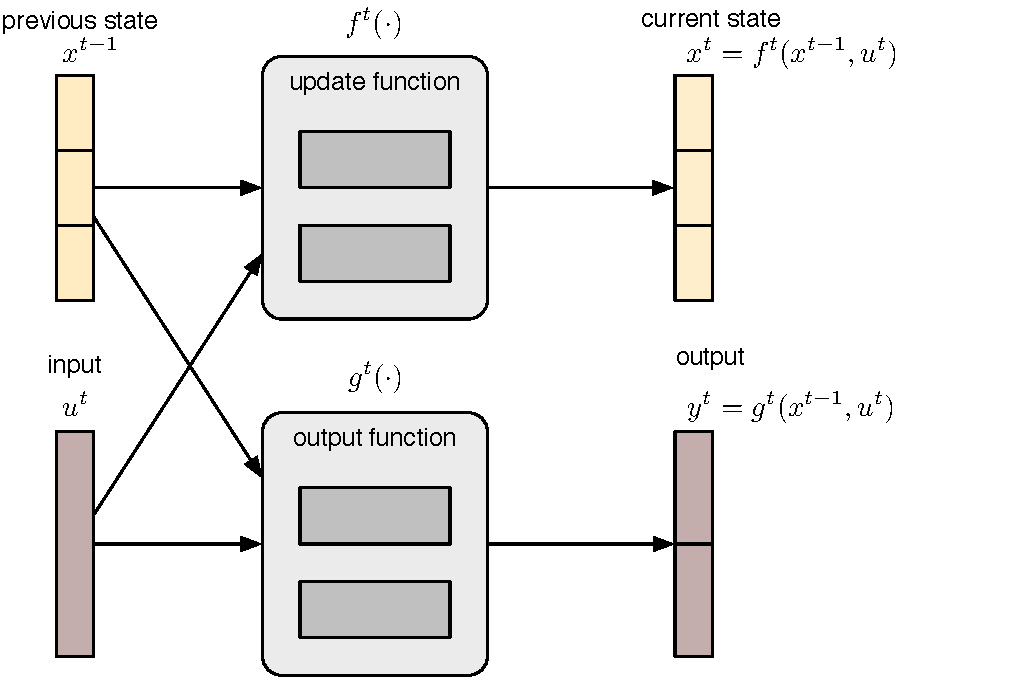
\includegraphics[width=0.8\textwidth]{figures/simulator-update-diagram-1}
  \caption{Simulator Update and Output Functions}
  \label{fig:update1}
\end{figure}

For a given time step~$t$, \figurename~\ref{fig:update1} illustrates a high-level view of the update and output functions used to compute the state $x^t$ and output $y^t$ from the previous state $x^{t-1}$ and current input $u^t$.

\begin{align}
x^t &= f^t(x^{t-1}, u^t) \label{eq:update} \\
y^t &= g^t(x^{t-1}, u^t) \label{eq:output}
\end{align}

\subsubsection{Partitioning by Process}
\label{sec:partitioning}

The state~$x$ consists of two types of components, \emph{process-specific state} updated only by the corresponding process and \emph{shared state} updated by more than one process.

\begin{figure}[hbtp]
  \centering
  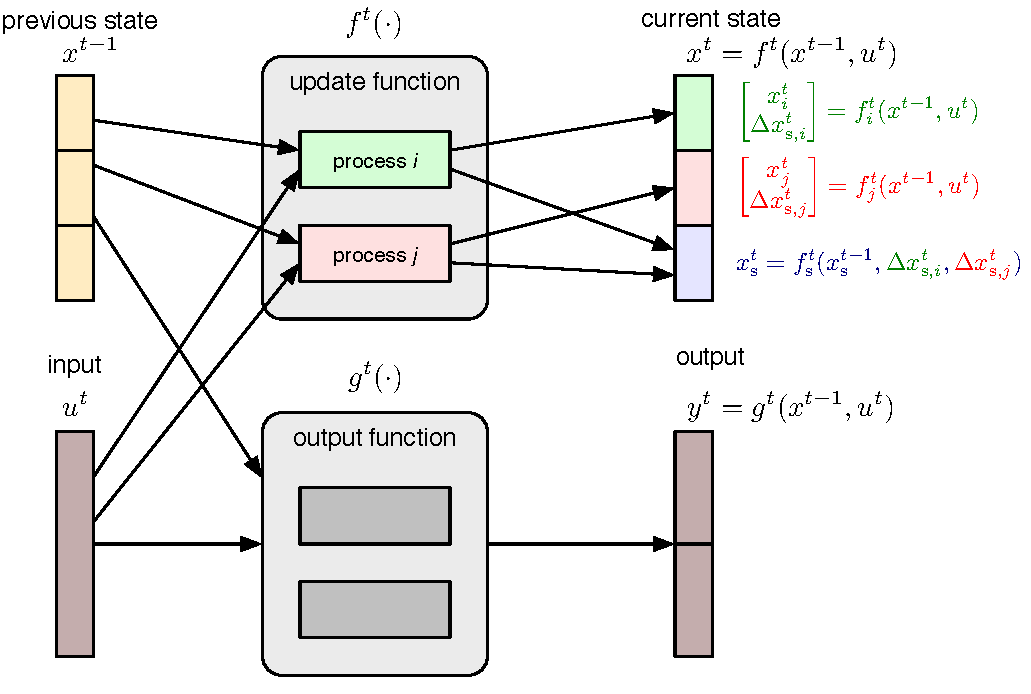
\includegraphics[width=0.8\textwidth]{figures/simulator-update-diagram-5}
  \caption{States and Update Functions Partitioned by Process}
  \label{fig:update5}
\end{figure}

\begin{figure}[hbtp]
  \centering
  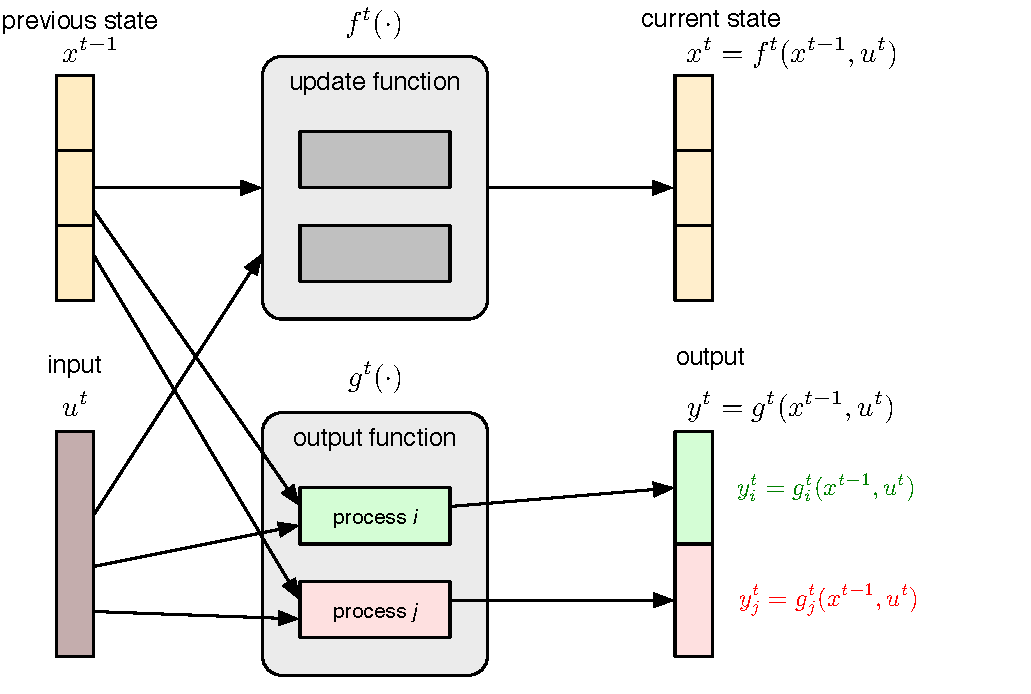
\includegraphics[width=0.8\textwidth]{figures/simulator-update-diagram-7}
  \caption{Outputs and Output Functions Partitioned by Process}
  \label{fig:update7}
\end{figure}

The overall update and output functions $f(\cdot)$ and $g(\cdot)$ are partitioned by process, as is the process-specific portion of the state and the output $y$ itself. For a simulator with two process $i$ and $j$, both of which execute in a single time step (no delay between trigger and finalize), \figurename~\ref{fig:update5} and \figurename~\ref{fig:update7} illustrate the process-specific update and output functions, respectively. Note that both processes can participate in updating the shared state $x_s^t$, by computing \emph{shared state updates}, namely $\Delta x_{s,i}^t$ and $\Delta x_{s,j}^t$ which are then applied together.

\subsubsection{Process Timing}
\label{sec:timing}

Each process \emph{triggers} at specified time steps and then \emph{finalizes} at later time steps based on the duration of the execution of the process. The trigger time determines what information is available as input to the process when it begins and the finalize time determines when modifications to the state performed by the process are available to be seen by other processes.
The timing of each process is controlled by the following three parameters:
\begin{itemize}
\item the time $t_0$ at which the process is first triggered,
\item the time $f$ between consecutive triggers of the process, controlling the frequency with which the process executes, and
\item the execution time $\tau$ that determines the amount of time between when the process triggers and when it finalizes.\footnote{Note that multiple executions of a process can overlap in time. That is, a second instance of a process can be triggered before the first has completed and been finalized.}
\end{itemize}


\begin{figure}[hbtp]
  \centering
  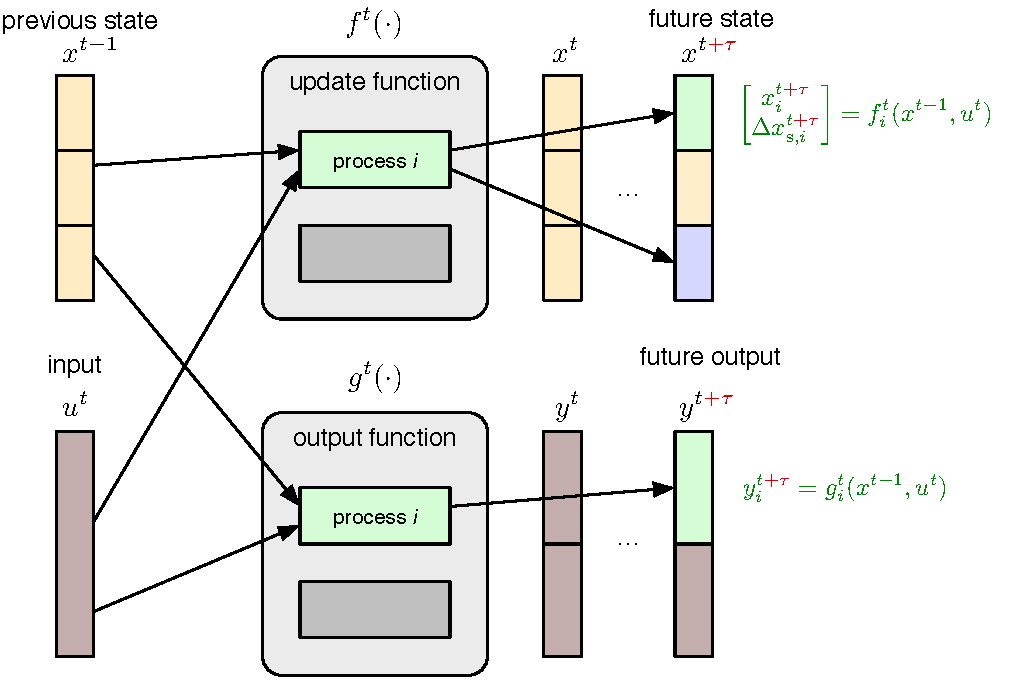
\includegraphics[width=0.8\textwidth]{figures/simulator-update-diagram-delay}
  \caption{Process with Run-time $\tau$}
  \label{fig:updatetau}
\end{figure}

Figures~\ref{fig:update5} and \ref{fig:update7} assumed a simplified context in which all processes are finalized in the same time step in which they are triggered (i.e. $\tau = 0$), which need not be the case. \figurename~\ref{fig:updatetau} illustrates the general form of the update and output functions for a process, where there is an arbitrary delay of $\tau$ time steps between when it is triggered and when it is finalized. In this case, it is the state and output at time $t+\tau$, rather than at~$t$, that are affected by the process triggered at time~$t$.

\subsubsection{Simulation Runs and Inputs}

It is often the case that we want to compare multiple runs of a simulation in which one or more input parameters are being varied across the runs. \mpsim{} is structured to allow multiple simulation runs with their inputs and outputs to be organized together in a \emph{simulation batch}. This batch can be organized as a simple one-dimensional list of runs, or more generally as a multi-dimensional collection of runs, where multiple inputs are being varied and we want to simulate all combinations of the inputs.

Note that the only difference between the runs in a simulation batch is the set of inputs used. Each run begins with the same initial state, determined at the time the simulator object is instantiated.

Since many of the inputs for a simulation may be constant from run to run, or even from time step to time step, \mpsim{} provides mechanisms for constructing and updating these portions of the input variable only as needed in order to make most efficient use of memory and computational resources. Depending on the context, input data on disk can be loaded at each step as needed, or pre-loaded into memory during initialization to speed up execution.

\subsubsection{Output Post-Processing}

Outputs can be written to disk during the simulation run or collected in memory to be handled by post-run processing code. This post-run processing code is typically used to generate summary reporting and visualizations of the simulation results.


%%------------------------------------------
\clearpage
\section{\mpsim{} Reference}
\label{sec:mpsim_ref}

This section provides a reference to the various classes and functions included in the \mpsim{} framework, with details of the object properties, function and method names, and input and output arguments.

\subsection{Notational Conventions}

Several notational conventions for variable, property, and field names are used throughout the code and this manual and are summarized in Table~\ref{tab:conventions}.

\begin{table}[!ht]
\centering
\begin{threeparttable}
\caption{Notational Conventions}
\label{tab:conventions}
\footnotesize
\begin{tabular}{lp{0.7\textwidth}}
\toprule
name & description \\
\midrule
\multicolumn{2}{l}{\emph{Values}} \\
~~\inputdir{}\tnote{\dag}	& path to base directory for input files \\
~~\outputdir{}\tnote{\dag}	& path to base directory for output files \\
~~\workdir{}\tnote{\dag}	& path to base directory for temporary work files \\
~~\simname{} 	& simulation name used to address input, output and temporary work files\\
~~\siminputdir{}	& path to simulation-specific directory for input files, constructed as \siminputdirpath {} \\
~~\simoutputdir{}	& path to simulation-specific directory for output files, constructed as \simoutputdirpath {} \\
~~\simworkdir{}	& path to simulation-specific directory for temporary work files, constructed as \simworkdirpath {} \\
\midrule
\multicolumn{2}{l}{\emph{Variable, Property and Field Names}} \\
\code{~~sim}	& simulator object \\
\code{~~sim\_name}, \code{sim.name}	& simulation name \simname{} \\
\code{~~sim\_inputdir}	& path to simulation-specific input directory \siminputdir{} \\
\code{~~sim\_outputdir}	& path to simulation-specific output directory \simoutputdir{} \\
\code{~~sim\_workdir}	& path to simulation-specific work directory \simworkdir{} \\
\code{~~r}	& index(es) of current run, 1-D cell array of scalars \\
\code{~~t}	& index of current simulation time step \\
\code{~~idx}	& index of process update (trigger or finalize) instance \\
\code{~~x}	& simulator state, $x$, see Section~\ref{sec:x} \\
\code{~~u}	& current input struct, $u^t$, see Section~\ref{sec:u} \\
\code{~~y}	& struct of all outputs, $y$, see Section~\ref{sec:y} \\
\code{~~ps}	& process object \\
\code{~~ps\_name}, \code{ps.name}	& name of process object \\
\code{~~x\_ps}	& process-specific portion of simulator state, $x_i$ \\
\code{~~y\_ps}	& process-specific output, $y_i$ \\
\code{~~sx}	& shared state object \\
\code{~~sx\_name}, \code{sx.name}	& name of shared state object \\
\code{~~sx\_update}	& shared state update for a single shared state object, struct array with fields \codeq{op} and \codeq{val} \\
\code{~~sx\_updates}	& struct of shared state updates for multiple shared state objects, with each update in a field named according the corresponding shared state name \\
\bottomrule
\end{tabular}
\begin{tablenotes}
 \scriptsize
 \item [\dag] {Specified in the \code{mpsim\_config.m} file found in \mpsimpath{/lib}, and set to \code{\textquotesingle{}}\mpsimpath{/sim\_data}\code{\textquotesingle{}} by default.}
\end{tablenotes}
\end{threeparttable}
\end{table}


\subsection{\mpsim{} Configuration -- {\tt mpsim\_config}}
\label{sec:mpsimconfig}

\mpsim{} configuration consists of paths to base directories for input, output and temporary work files, denoted by \inputdir{}, \outputdir{} and \workdir{}, respectively. These are determined by the values of the \code{inputdir}, \code{outputdir} and \code{workdir} variables in the \code{mpsim\_config.m} file found in \mpsimpath{/lib}. These are string value variables containing the absolute or relative path to the corresponding directory. If left blank, the default \inputdir{} points to \mpsimpath{/sim\_data}. Likewise, the default behavior for \outputdir{} and \workdir{} is to set each equal to \inputdir{}.

Upon installation of \mpsim{} these values are all blank, but they can be changed for a given \mpsim{} installation by editing the appropriate lines in the \code{mpsim\_config.m} file. The only lines that should be modified are those that define the \code{inputdir}, \code{outputdir} and \code{workdir} variables. \emph{Note that this configuration affects all simulations run by this installation of \mpsim{}}.

Within these base directories, which may or may not point to the same directory, files are organized by simulation batch. For a simulation named \simname{}, \mpsim{} will expect to find the input files in the simulation-specific directory for input files, namely \siminputdirpath{}, which is also denoted by \siminputdir{}. This path is passed to methods that need access to input files. Similarly, the simulation writes any output files to \simoutputdirpath{}, and any temporary working files to \simworkdirpath{}, denoted \simoutputdir{} and \simworkdir{}, respectively. These paths are likewise passed to methods that need access to the corresponding files.
This design keeps all data files for a given simulation batch together under a directory whose name is the simulation name.

\subsection{Structure of Simulator State $x$}
\label{sec:x}

The simulator state $x$, as described in Section~\ref{sec:partitioning}, is partitioned into two parts, the shared part and the process-specific part. It is implemented as a struct \code{x} with the shared part contained in the \code{shared} field and the process-specific part contained in fields named according to name of the corresponding process object. The \code{shared} field is also a struct whose field names correspond to the names of the various shared state objects. This structure is summarized in Table~\ref{tab:x_struct}.

\begin{table}[!h]
\centering
\begin{threeparttable}
\caption{Structure of Simulator State $x$}
\label{tab:x_struct}
\footnotesize
\begin{tabular}{lp{0.77\textwidth}}
\toprule
name & description \\
\midrule
\code{x}	& full simulator state struct \\
\code{~~.(ps\_name)}	& struct containing arbitrary fields defined by process object identified by name \code{ps\_name} \\
\code{~~.shared}	& struct of shared state fields \\
\code{~~~~.(sx\_name)}	& struct containing arbitrary fields defined by shared state object identified by name \code{sx\_name} \\
\bottomrule
\end{tabular}
\end{threeparttable}
\end{table}

For example, suppose a process named \codeq{foo} defines its process specific state as a struct with a field named \codeq{bar}. Then the value of this piece of the state would be found in \code{x.foo.bar}. Similarly, if a shared state object named \codeq{baz} defined a field named \codeq{buz}, the value of that piece of the state would be found in \code{x.shared.baz.buz}.

Note that it is only the shared state \emph{value} that is contained in the shared portion of the state \code{x}, not the shared state \emph{object} used to manage and update it.

\subsection{Structure of Simulator Input $u$}
\label{sec:u}

The input $u$, also illustrated in Section~\ref{sec:partitioning}, is an arbitrary user-defined value. More specifically, $u^t$ is an arbitrary user-defined set of information made available to the simulator at time step~$t$. It is assembled at each time step from multiple sources, including collections of data loaded at the beginning of the simulation batch, at the beginning of the current simulation run, and at the current time step. Each of these 3 collections of data can consist of a global portion associated with the overall simulation as well as portions associated with specific processes triggered at time~$t$..

The user does not define the input $u^t$ directly, but indirectly, by implementing simulator and simulator process methods\footnote{Namely \code{preload\_sim\_inputs},  \code{preload\_run\_inputs} and  \code{load\_current\_inputs}. See Sections~\ref{sec:mpsim_override_methods} and \ref{sec:ps_override_methods} for details.} to handle the various preloading and loading options. \mpsim{} then assembles $u^t$ automatically from the collections of data provided by these methods. Table~\ref{tab:input_return_args} describes the various variables that are defined and returned by these methods.

\begin{table}[!ht]
\centering
\begin{threeparttable}
\caption{Return Arguments for Input Loading Methods\tnote{*}}
\label{tab:input_return_args}
\footnotesize
\begin{tabular}{lp{0.68\textwidth}}
\toprule
name & description \\
\midrule
\code{thissim}	& struct of input data pre-loaded at beginning of simulation batch \\
\code{thisrun}	& struct of input data pre-loaded at beginning of simulation run \\
\code{thisidx}	& struct of input data loaded at current time step \\
\code{byrun}	& struct array of input data pre-loaded at beginning of simulation batch, indexed by run \\
\code{byt}	& struct array of input data pre-loaded at beginning of simulation batch or run, indexed by time index \code{t} \\
\code{byidx}	& struct array of input data pre-loaded at beginning of simulation batch or run, indexed by process update instance \code{idx} \\
\code{byboth}	& struct array of input data pre-loaded at beginning of simulation batch, indexed by both run \code{r} and time step \code{t}, or by both run \code{r} and process update instance \code{idx}\tnote{\dag} \\
\midrule
\multicolumn{2}{p{0.96\textwidth}}{The input struct \code{u}, as passed to the \code{ps.update()} functions, includes data loaded by these methods\tnote{*}. That is, all fields from the following return args of these methods are copied into input struct \code{u}:} \\
\code{~~thissim} & \\
\code{~~thisrun} & \\
\code{~~thisidx} & \\
\code{~~byrun(r\lcb{}:\rcb{})} & for current simulation run \code{r} \\
\code{~~byt(t)} & for current time step \code{t} \\
\code{~~byidx(idx)} & for current process update instance \code{idx} \\
\code{~~byboth(r\lcb{}:\rcb{},t)} & for current simulation run \code{r} and time step \code{t}, or \\
\code{~~byboth(r\lcb{}:\rcb{},idx)} & for current simulation run \code{r} and process update instance \code{idx} \\
\bottomrule
\end{tabular}
\begin{tablenotes}
 \scriptsize
 \item [*] {Namely the \code{preload\_sim\_inputs},  \code{preload\_run\_inputs} and  \code{load\_current\_inputs} methods of the simulator and process classes.}
 \item [\dag] {Depending on whether it is returned by a simulator method or a process method.}
\end{tablenotes}
\end{threeparttable}
\end{table}

This design helps to prevent the user from accidentally providing a process with information that should not be available at the current time step. The key detail to keep in mind when implementing these methods is that the fields in the provided data are simply copied to \code{u} when it is assembled, so each type of information should use a unique field name to avoid data getting inadvertently clobbered.


% \begin{Code}
% sim
%   .u_preloaded
%     .sim
%       .thissim          - sim.preload_sim_inputs()
%       .byrun(r{:})      - sim.preload_sim_inputs()
%       .byt(t)           - sim.preload_sim_inputs()
%       .byboth(r{:},t)   - sim.preload_sim_inputs()
%       .thisrun
%         .thisrun        - sim.preload_run_inputs()
%         .byt(t)         - sim.preload_run_inputs()
%     .(ps_name)
%       .thissim          - ps.preload_sim_inputs()
%       .byrun(r{:})      - ps.preload_sim_inputs()
%       .byidx(idx)       - ps.preload_sim_inputs()
%       .byboth(r{:},idx) - ps.preload_sim_inputs()
%       .thisrun
%         .thisrun        - ps.preload_run_inputs()
%         .byidx(t)       - ps.preload_run_inputs()
% 
%   .preload_sim_inputs()
%   .preload_run_inputs()
%   .load_current_inputs()
%   .preload_all_sim_inputs() - calls sim.preload_sim_inputs(),
%                                      ps.preload_sim_inputs()
%   .preload_all_run_inputs() - calls sim.preload_run_inputs(),
%                                      ps.preload_run_inputs()
%   .input() - calls sim.load_current_inputs(), ps.load_current_inputs()
% ps
%   .input()         - modify inputs?
% \end{Code}
  
\subsection{Structure of Simulator Output $y$}
\label{sec:y}

At each time step the simulator may produce an output $y$, or more precisely $y^t$. Some portion of these outputs may be written to output files directly by the \code{output} method of a process while other portions are collected in memory inside the simulator object for post-processing (e.g. saving, printing, plotting) by a \code{post\_run} method. This output is stored in \code{sim.y} as follows, where \code{r} is the index of the run and \code{idx} is the index of the process update instance.

\begin{table}[!h]
\centering
\begin{threeparttable}
\caption{Structure of Simulator Output Struct}
\label{tab:y}
\footnotesize
\begin{tabular}{lp{0.66\textwidth}}
\toprule
name & description \\
\midrule
\code{y}	& full simulator output struct \\
\code{~~.(ps\_name)(r\lcb{}:\rcb{}, idx)}	& struct containing arbitrary fields defined by process \code{output} methods, identified by corresponding process name \code{ps\_name} and indexed by the current run \code{r} and process update instance \code{idx} \\
\bottomrule
\end{tabular}
\end{threeparttable}
\end{table}

% \begin{Code}
% sim
%   .y
%     .(ps_name)(r{:},idx) - ps.output()
%   .out_args
%     .(ps_name)
% 
%   .output()
% \end{Code}

%\clearpage
\subsection{Simulator Class -- {\tt mpsim}}
\label{sec:mpsim}

The \code{mpsim} class serves as the abstract base class for all simulator objects and provides the top-level interface to the user for running simulations. The properties and methods are listed in Tables~\ref{tab:mpsim_properties} and \ref{tab:mpsim_methods}. Further detail is provided in the following two sections for the public methods and for the private methods that are intended to be implemented or overridden by a subclass.

\begin{table}[!ht]
\centering
\begin{threeparttable}
\caption{Properties of \code{mpsim}}
\label{tab:mpsim_properties}
\footnotesize
\begin{tabular}{lp{0.73\textwidth}}
\toprule
name & description \\
\midrule
\multicolumn{2}{l}{\emph{Public Properties}} \\
\code{~~l}	& length of simulation time step\tnote{*} \\
\code{~~units}	& string value of units of \code{l}, for user reference only (e.g. \codeq{minutes} or \codeq{hours}) \\
\code{~~name}	& name of current simulation batch \simname{}, used to construct paths to directories with simulation data \\
\code{~~processes}	& cell array of process objects registered with simulator \\
\code{~~R}	& scalar or vector of dimension of runs in current simulation batch \\
\code{~~T}	& number of simulation time steps per run in current simulation batch \\
\code{~~r}	& index(es) of current run, 1-D cell array of scalars \\
\code{~~t}	& index of current simulation time step \\
\code{~~x}	& simulator state $x$, with process-specific portions in  \code{x.(ps\_name)} and shared portions in \code{x.shared.(sx\_name)}, see Section~\ref{sec:x} \\
\code{~~y}	& struct containing outputs generated during simulation, see Section~\ref{sec:y} \\
\code{~~verbose}	& (0--3), option specifying level of detailed progress to be printed to screen during a simulation run (default = 0, i.e. no output) \\
\code{~~inspect}	& (0, 1), option to automatically enter debugger at end of \code{input} method to allow user to inspect the input struct (default~=~0) \\
\code{~~post\_run\_on}	& (0, 1) option controlling whether or not \code{post\_run} method is executed (default~=~1) \\
\code{~~options}	& struct containing custom options passed to \code{run}; includes all options passed except the standard \code{R}, \code{T}, \code{verbose}, \code{inspect} and \code{post\_run\_on} which are modified directly in the corresponding \code{sim} properties \\
\midrule
\multicolumn{2}{l}{\emph{Private Properties}} \\
\code{~~config}	& struct of paths to base directories for input, output and temporary work files in fields \code{inputdir}, \code{outputdir} and \code{workdir}, respectively, as specified in \code{mp\_sim\_config}\\
\code{~~out\_args}	& current set of arguments, as provided by \code{ps.update()}, to be passed to \code{sim.output()} \\
\code{~~shared\_x\_objects}	& struct of shared state objects used to update shared portion of state $x$, fields named according to name of corresponding shared state object\tnote{\dag} \\
\code{~~shared\_x\_names}	& cell array of names of shared state fields/objects \\
\code{~~u\_preloaded}	& struct containing inputs pre-loaded at beginning of simulation batch or current run\tnote{\ddag} \\
\code{~~x0}	& copy of initial simulator state $x$ made before first run \\
\code{~~x\_updates}	& updates to simulator state to be applied when processes finalize \\
\bottomrule
\end{tabular}
\begin{tablenotes}
 \scriptsize
 \item [*] {The values of \code{ps.f}, \code{ps.t0}, and \code{ps.tau}, for all processes \code{ps}, must be evenly divisible by \code{sim.l}.}
 \item [\dag] {Object at \code{sim.shared\_x\_objects.(sx\_name)} is used to update shared state value at \code{sim.x.shared.(sx\_name)}}.
 \item [\ddag] {Pre-loaded inputs are defined by the \code{preload\_sim\_inputs} and \code{preload\_run\_inputs} methods of the simulator and/or process objects.}
\end{tablenotes}
\end{threeparttable}
\end{table}

\begin{table}[!h]
\centering
\begin{threeparttable}
\caption{Methods of \code{mpsim}}
\label{tab:mpsim_methods}
\footnotesize
\begin{tabular}{lp{0.66\textwidth}}
\toprule
name & description \\
\midrule
\multicolumn{2}{l}{\emph{Public Methods}} \\
\code{~~mpsim}	& simulator object constructor (called indirectly by subclass) \\
\code{~~add\_shared\_state}	& add a shared state object and its initial value to the simulator \\
\code{~~display}	& display information about simulation properties and processes \\
\code{~~register\_process}	& register a process with the simulator \\
\code{~~reset}	& set time index $t$ to 1, reset simulator state to initial value \\
\code{~~run}	& execute specified runs of the simulation \\
\midrule
\multicolumn{2}{l}{\emph{Private Methods -- override as needed}} \\
\code{~~initialize}	& set default simulator properties, create \& add any shared states, create \& register processes \\
\code{~~load\_current\_inputs}	& load inputs for current time step \\
\code{~~preload\_run\_inputs}	& pre-load inputs at beginning of each simulation run \\
\code{~~preload\_sim\_inputs}	& pre-load inputs at beginning of simulation \\
\code{~~post\_run}	& post-process simulation outputs \\
\midrule
\multicolumn{2}{l}{\emph{Private Methods -- should not need to override}} \\
\code{~~apply\_ps\_x}	& apply queued update to process-specific state \\
\code{~~apply\_run\_options}	& copy set of run options to simulator object \\
\code{~~apply\_shared\_x}	& apply queued update for given process to shared state \\
\code{~~increment\_run}	& increment simulation run counter in \code{sim.r} \\
\code{~~initialize\_output}	& initialize the output cache in \code{sim.y} \\
\code{~~input}	& construct input struct \code{u} for current run and time step \\
\code{~~inputdir}	& return path to a simulation-specific input file or directory \\
\code{~~output}	& collect output from finalizing processes that provide it \\
\code{~~outputdir}	& return path to a simulation-specific output file or directory \\
\code{~~preload\_all\_run\_inputs}	& cache results of \code{preload\_run\_inputs} for simulator and processes \\
\code{~~preload\_all\_sim\_inputs}	& cache results of \code{preload\_sim\_inputs} for simulator and processes \\
\code{~~queue\_out\_args}	& push arguments to pass from \code{ps.update()} to \code{ps.output()} to corresponding FIFO queue \\
\code{~~queue\_ps\_x}	& push updated process-specific state to corresponding FIFO queue\\
\code{~~queue\_shared\_x}	& push shared state updates to corresponding FIFO queue \\
\code{~~step}	& update state for finalizing processes and increment time step \\
\code{~~update}	& call \code{ps.update()} for processes triggered at current time step \\
\code{~~workdir}	& return path to a simulation-specific work file or directory \\
\bottomrule
\end{tabular}
% \begin{tablenotes}
%  \scriptsize
%  \item [\dag] {Footnote.}
% \end{tablenotes}
\end{threeparttable}
\end{table}

\subsubsection{Public Methods}
\label{sec:mpsim_public_methods}

\paragraphtt{mpsim}
This is the constructor for the simulator object and is always called indirectly by the constructor of the subclass, never directly by the user. It takes no input arguments. After initializing configuration information via \code{mpsim\_config} it calls the \code{initialize} method.
\begin{Code}
sim = mpsim()
\end{Code}
Subclasses of \code{mpsim} will typically override the \code{initialize} method, but inherit the constructor itself without modification.

\paragraphtt{add\_shared\_state}
Adds the specified shared state object \code{sx} to the simulator.
\begin{Code}
sim = sim.add_shared_state(sx)
\end{Code}

\clearpage
\paragraphtt{display}
Displays the details of the simulator object, including its properties and processes. Automatically called to display the object when a simulator object is the result of a statement (e.g. on the command-line) that is not terminated with a semicolon.
\begin{Code}
sim.display()
sim
\end{Code}

\paragraphtt{register\_process}
Checks compatibility of the process and simulator timing parameters, initializes the private data structures for tracking state updates and output arguments for the process, and registers the process object \code{ps} with the simulator.
\begin{Code}
sim = sim.register_process(ps)
\end{Code}

\paragraphtt{reset}
Sets the time index \code{sim.t} back to 1 and resets the simulator state to the initial value, including the values of all shared state objects. Called before the start of each new run.
\begin{Code}
sim = sim.reset()
\end{Code}

\paragraphtt{run}
Executes the specified runs of the simulation using the input, output and work directories and files corresponding to the simulation batch indicated by \code{sim\_name}, and the specified \mpsim{} options.
\begin{Code}
sim = sim.run(sim_name, opt_struct)
sim = sim.run(sim_name, opt1_name, opt1_val, ...)
sim = sim.run(sim_name, opt1_name, opt1_val, ... opt_struct)
\end{Code}
If the \codeq{r} option is not specified, it executes all runs specified by the \code{R} attribute of the simulation, which can be set at run time by the \codeq{R} option.

\mpsim{} options can be specified as a struct (\code{opt\_struct}) or a set of name/value pairs (\code{opt1\_name}, \code{opt1\_val}, etc) or a combination of both. Table~\ref{tab:mpsim_run_options} lists the standard options that are available in the corresponding public attributes of the simulator object. All other options are considered custom options and are available in \code{sim.options}.

\begin{table}[!h]
\centering
\begin{threeparttable}
\caption{\mpsim{} Run Options}
\label{tab:mpsim_run_options}
\footnotesize
\begin{tabular}{lcp{0.73\textwidth}}
\toprule
name & default & description \\
\midrule
\codeq{verbose}	& 0	& integer from 0 to 4 specifying the level of detail of progress output printed during the simulation \\
\codeq{inspect}	& 0	& 1 to pause simulation at each step after construction of the input data \code{u} to allow inspection \\
\codeq{r}	& \emph{all}	& index(es) of single simulation run to execute (cell array) \\
\codeq{R}	& \code{sim.R}	& scalar or vector of dimension of runs to execute \\
\codeq{T}	& \code{sim.T}	& number of simulation time steps per run to execute \\
\bottomrule
\end{tabular}
% \begin{tablenotes}
%  \scriptsize
%  \item [\dag] {Footnote.}
% \end{tablenotes}
\end{threeparttable}
\end{table}


\subsubsection{Private Methods -- \emph{override as needed}}
\label{sec:mpsim_override_methods}

\paragraphtt{initialize} Sets the default values for the simulator properties \code{l}, \code{units}, \code{R} and \code{T}, creates and add any shared states, then creates and registers the process objects. This method \emph{must} be implemented in your \code{mpsim} subclass.
\begin{Code}
sim = sim.initialize()
\end{Code}

\paragraphtt{load\_current\_inputs}
Called at each time period to load inputs that are not process-specific (particularly in terms of timing). Returns an empty value by default, but can be overridden by the user to load data for run \code{r} and time \code{t} specific to their simulation.
\begin{Code}
thisidx = sim.load_current_inputs(sim_name, sim_inputdir, r, t)
\end{Code}

The input struct \code{u}, as passed to the \code{ps.update()} functions, includes the data loaded by this method at each time step. That is, in addition to data from other sources, all fields from \code{thisidx} are copied into input struct \code{u}. See Table~\ref{tab:input_return_args} for details on the return argument.

\paragraphtt{preload\_run\_inputs} Called at the beginning of each simulation run to pre-load inputs that are not process-specific (particularly in terms of timing). Returns empty values by default, but can be overridden by the user to load data for run \code{r} specific to their simulation.
\begin{Code}
[thisrun, byt] = sim.preload_run_inputs(sim_name, sim_inputdir, r)
\end{Code}

The input struct \code{u}, as passed to the \code{ps.update()} functions, includes data pre-loaded by this method at the beginning of each simulation run. That is, in addition to data from other sources, all fields from \code{thisrun} and \code{byt(t)} (for the current time step \code{t}) are copied into input struct \code{u}. See Table~\ref{tab:input_return_args} for details on the return arguments.

\paragraphtt{preload\_sim\_inputs} Called at the beginning of a simulation batch to pre-load inputs that are not process-specific (particularly in terms of timing). Returns empty values by default, but can be overridden by the user to load data specific to their simulation.
\begin{Code}
[thissim, byrun, byt, byboth] = ...
    sim.preload_sim_inputs(sim_name, sim_inputdir)
\end{Code}

The input struct \code{u}, as passed to the \code{ps.update()} functions, includes data pre-loaded by this method at the beginning of the simulation. That is, in addition to data from other sources, all fields from \code{thissim}, \code{byrun(r\lcb{}:\rcb{})}, \code{byt(t)}, and \code{byboth(r\lcb{}:\rcb{},t)} (for the current run \code{r} and time step \code{t}) are copied into input struct \code{u}. See Table~\ref{tab:input_return_args} for details on the return arguments.

\paragraphtt{post\_run} Simulation outputs are returned by the various process \code{output} methods during the execution of the simulation batch and collected in an output struct \code{y}, described in Table~\ref{tab:y}. This method is called after the execution of all runs is complete.\footnote{Unless the \codeq{post\_run\_on} option is set to 0.} Does nothing by default, but can be overridden by the user to post-process the outputs \code{y} specific to their simulation.
\begin{Code}
sim.post_run(y, sim_outputdir)
\end{Code}

% \subsubsection{Private Methods -- \emph{should not need to override}}
% \label{sec:mpsim_private_methods}
% 
% \paragraphtt{apply\_ps\_x}
% \hl{Description.}
% \begin{Code}
% sim = sim.apply_ps_x(ps_name)
% \end{Code}
% 
% \paragraphtt{apply\_run\_options}
% \hl{Description.}
% \begin{Code}
% sim = sim.apply_run_options(run_options)
% \end{Code}
% 
% \paragraphtt{apply\_shared\_x}
% \hl{Description.}
% \begin{Code}
% sim = sim.apply_shared_x(ps_name)
% \end{Code}
% 
% \paragraphtt{increment\_run}
% \hl{Description.}
% \begin{Code}
% done = sim.increment_run()
% \end{Code}
% 
% \paragraphtt{initialize\_output}
% \hl{Description.}
% \begin{Code}
% sim = sim.initialize_output()
% \end{Code}
% 
% \paragraphtt{input}
% \hl{Description.}
% \begin{Code}
% u = sim.input(sim_inputdir, r, t)
% \end{Code}
% 
% \paragraphtt{inputdir}
% \hl{Description.}
% \begin{Code}
% pathname = sim.inputdir(varargin)
% \end{Code}
% 
% \paragraphtt{output}
% \hl{Description.}
% \begin{Code}
% sim = sim.output(u, sim_outputdir, r, t)
% \end{Code}
% 
% \paragraphtt{outputdir}
% \hl{Description.}
% \begin{Code}
% pathname = sim.outputdir(varargin)
% \end{Code}
% 
% \paragraphtt{preload\_all\_run\_inputs}
% \hl{Description.}
% \begin{Code}
% sim = sim.preload_all_run_inputs(r)
% \end{Code}
% 
% \paragraphtt{preload\_all\_sim\_inputs}
% \hl{Description.}
% \begin{Code}
% sim = sim.preload_all_sim_inputs()
% \end{Code}
% 
% \paragraphtt{queue\_out\_args}
%
% \hl{Description.}
% \begin{Code}
% sim = sim.queue_out_args(ps_name, out_args)
% \end{Code}
% 
% \paragraphtt{queue\_ps\_x}
% \hl{Description.}
% \begin{Code}
% sim = sim.queue_ps_x(ps_name, x_ps)
% \end{Code}
% 
% \paragraphtt{queue\_shared\_x}
% \hl{Description.}
% \begin{Code}
% sim = sim.queue_shared_x(ps_name, sx_updates)
% \end{Code}
% 
% \paragraphtt{step}
% \hl{Description.}
% \begin{Code}
% sim = sim.step()
% \end{Code}
% 
% \paragraphtt{update}
% \hl{Description.}
% \begin{Code}
% sim = sim.update(x, u, sim_workdir, r, t)
% \end{Code}
% 
% \paragraphtt{workdir}
% \hl{Description.}
% \begin{Code}
% pathname = sim.workdir(varargin)
% \end{Code}
% 

\subsection{Shared State Class -- {\tt mpsim\_shared\_x}}
% \subsection{Shared State Classes -- {\tt mpsim\_shared\_x, mpsim\_shared\_x\_numeric, mpsim\_shared\_x\_queue}}
\label{sec:sharedstate}

The \code{mpsim\_shared\_x} class serves as the abstract base class for all shared state objects. The properties and methods are listed in Tables~\ref{tab:shared_state_properties} and \ref{tab:shared_state_methods}. Further detail is provided in the following two sections for the public methods and for the private methods that are intended to be implemented or overridden by a subclass.

\begin{table}[!h]
\centering
\begin{threeparttable}
\caption{Properties of \code{mpsim\_shared\_x}}
\label{tab:shared_state_properties}
\footnotesize
\begin{tabular}{lp{0.76\textwidth}}
\toprule
name & description \\
\midrule
\multicolumn{2}{l}{\emph{Public Properties}} \\
\code{~~name}	& name of shared state object (typically denoted \code{sx\_name}) \\
\midrule
\multicolumn{2}{l}{\emph{Private Properties}} \\
\code{~~initial\_value}	& starting value for the shared state at beginning of simulation batch, specified by \code{initialize} method\tnote{\dag}	\\
\code{~~value}	& current value of the shared state, type is determined by the \code{initialize} method, and value is updated by the \code{update} method \\
\bottomrule
\end{tabular}
\begin{tablenotes}
 \scriptsize
 \item [\dag] {By convention, the \code{initialize} method is designed to load the data for the initial value from a file, located in \siminputdir{/shared\_states}, with the same name as the shared state object.}
\end{tablenotes}
\end{threeparttable}
\end{table}

\begin{table}[!h]
\centering
\begin{threeparttable}
\caption{Methods of \code{mpsim\_shared\_x}}
\label{tab:shared_state_methods}
\footnotesize
\begin{tabular}{lp{0.75\textwidth}}
\toprule
name & description \\
\midrule
\multicolumn{2}{l}{\emph{Public Methods}} \\
\code{~~mpsim\_shared\_x}	& shared state object constructor (called indirectly by subclass) \\
\midrule
\multicolumn{2}{l}{\emph{Private Methods -- override as needed}} \\
\code{~~initialize}	& initialize value of shared state \\
\code{~~update}	& update value of shared state based on the  \\
\bottomrule
\end{tabular}
% \begin{tablenotes}
%  \scriptsize
%  \item [\dag] {Footnote.}
% \end{tablenotes}
\end{threeparttable}
\end{table}

The shared state mechanism in \mpsim{} involves three types of data. The first is the \emph{shared state value} found directly in the simulator state, that is, in \code{sim.x.shared.(sx\_name)}. These values are available directly to the process \code{update} and \code{output} methods as read-only values. On the other hand, each of these values is updated only indirectly, by the corresponding \emph{shared state object}. In particular, a process \code{update} method may return a set of \emph{shared state updates} (\code{sx\_updates}) that are automatically applied to the state at the proper time via the \code{update} method of the corresponding shared state object. These shared state updates consist of an update value and an operation used to apply that value, for instance, adding or subtracting a value to an inventory, or pushing or popping a value from a queue.

\subsubsection{Public Method}
\label{sec:sx_public_methods}

\paragraphtt{mpsim\_shared\_x}
This is the constructor for shared state objects and is always called indirectly by the constructor of the subclass, never directly by the user. The only input is the name of the shared state object \code{sx\_name}.
\begin{Code}
sx = mpsim_shared_x(sx_name)
\end{Code}

% \paragraphtt{display}
% \hl{Description.}
% \begin{Code}
% 
% \end{Code}
% 

\subsubsection{Private Methods -- \emph{override as needed}}
\label{sec:sx_override_methods}

\paragraphtt{initialize}
This method is responsible for setting the initial value of the shared state and \emph{must} be implemented in your \code{mpsim\_shared\_x} subclass.
\begin{Code}
starting_value = sx.initialize(sim_inputdir, sim_name)
\end{Code}

By convention, the \code{initialize} method is designed to load the data for the initial value from a file, located in \siminputdir{/shared\_states}, with the same name as the shared state object.

\paragraphtt{update}
This method is responsible for applying a shared state update (\code{sx\_update}) to the value of the shared state and \emph{must} be implemented in your \code{mpsim\_shared\_x} subclass.
\begin{Code}
sx.update(sx_update)
\end{Code}

The shared state update \code{sx\_update} is a 1-dimensional struct array with fields \codeq{op} and \codeq{val}, containing the operation and value, respectively to be applied. If \code{sx\_update} has more than one element, \code{update} should apply each of them in order.

\subsubsection{Subclasses -- {\tt mpsim\_shared\_x\_numeric, mpsim\_shared\_x\_queue}}
\label{sec:sx_subclasses}

\paragraphtt{mpsim\_shared\_x\_numeric}
This subclass of \code{mpsim\_shared\_x} implements a shared state whose value is a numerical scalar or array. The \code{initialize} method uses the built-in \code{load} function to load the initial value of the shared state from a text file, located in \siminputdir{/shared\_states}, with the same name as the shared state object and with a \codeq{.txt} extension. For example, a shared state object named \codeq{inventory} would load its initial value from \siminputdir{/shared\_states/inventory.txt}.

\begin{table}[!h]
\centering
\begin{threeparttable}
\caption{Update Operations (\code{sx\_update.op}) for \code{mpsim\_shared\_x\_numeric}}
\label{tab:mpsim_shared_x_numeric}
\footnotesize
\begin{tabular}{cl}
\toprule
operation & description \\
\midrule
\codeq{+}	& add update value to current value \\
\codeq{-}	& subtract update value from current value \\
\codeq{*}	& multipy current value by update value \emph{(matrix multiply)} \\
\codeq{/}	& divide current value by update value \emph{(matrix divide)} \\
\codeq{\^{}}	& raise current value to power of update value \emph{(matrix exponent)} \\
\codeq{.*}	& multipy current value by update value \emph{(elementwise)} \\
\codeq{./}	& divide current value by update value \emph{(elementwise)} \\
\codeq{.\^{}}	& raise current value to power of update value \emph{(elementwise)} \\
\codeq{=}	& replace current value with update value \\
\bottomrule
\end{tabular}
% \begin{tablenotes}
%  \scriptsize
%  \item [\dag] {Footnote.}
% \end{tablenotes}
\end{threeparttable}
\end{table}

The valid update operations are shown in Table~\ref{tab:mpsim_shared_x_numeric}. So, for example, if the input text file contains a simple scalar, the following defines an update of length 2 that specifies an increment of the current value by 43, followed by doubling it.
\begin{Code}
sx_update = struct('op', {'+', '*'}, 'val', {43, 2});
\end{Code}
The \code{mpsim\_shared\_x\_numeric} class can typically be used without any further subclassing.

\paragraphtt{mpsim\_shared\_x\_queue}
This subclass of \code{mpsim\_shared\_x} implements a shared state whose value is a FIFO queue of arbitrary data. Due to the potentially arbitrary nature of the data in the initial queue, the \code{initialize} method calls a function that returns the initial value of the shared state. The function is located in an M-file in \siminputdir{/shared\_states} with the same name as the shared state object. For example, a shared state object named \codeq{test\_queue} would load its initial value using the \code{test\_queue} function found in \siminputdir{/shared\_states/test\_queue.m}.

\begin{table}[!h]
\centering
\begin{threeparttable}
\caption{Update Operations (\code{sx\_update.op}) for \code{mpsim\_shared\_x\_queue}}
\label{tab:mpsim_shared_x_queue}
\footnotesize
\begin{tabular}{cl}
\toprule
operation & description \\
\midrule
\codeq{+}	& push update values to the queue, update values can be scalar or cell array  \\
\codeq{-}	& pop values from the queue, where update value gives number of elements to pop \\
\bottomrule
\end{tabular}
% \begin{tablenotes}
%  \scriptsize
%  \item [\dag] {Footnote.}
% \end{tablenotes}
\end{threeparttable}
\end{table}

The valid update operations are shown in Table~\ref{tab:mpsim_shared_x_queue}. So, the following defines an update of length 1 that specifies pushing two elements to the queue: the matrix \code{[1 2; 3 4]}, then the string \codeq{Hello FIFO!}.

\begin{Code}
sx_update = struct('op', '+', 'val', {{[1 2; 3 4], 'Hello FIFO!'}});
\end{Code}
The \code{mpsim\_shared\_x\_queue} class can typically be used without any further subclassing.

\subsection{Simulator Process Class -- {\tt mpsim\_process}}
\label{sec:mpsimprocess}

The \code{mpsim\_process} class serves as the abstract base class for all process objects, which define the basic tasks and behaviors performed by the simulator. The properties and methods are listed in Tables~\ref{tab:mpsim_process_properties} and \ref{tab:mpsim_process_methods}. The parameters, $t_0$, $f$ and $\tau$, discussed in Section~\ref{sec:timing}, are properties of the process object and define the timing of the triggering and finalizing of the process. In summary, the process triggers at time step $(t_0+fi)/l$ and finalizes at $(t_0+\tau+fi)/l$, for $i = 1, 2, \dots n_{\rm idx}$, where $l$ is the length of the simulation time step (\code{sim.l}).

Further detail is provided in the following two sections for the public methods and for the private methods that are intended to be implemented or overridden by a subclass.

\begin{table}[!ht]
\centering
\begin{threeparttable}
\caption{Properties of \code{mpsim\_process}}
\label{tab:mpsim_process_properties}
\footnotesize
\begin{tabular}{lp{0.8\textwidth}}
\toprule
name & description \\
\midrule
\multicolumn{2}{l}{\emph{Public Properties}} \\
\code{~~name}	& name of process  	\\
\code{~~f}	& $f$, amount of time between instances of process update\tnote{\dag}	\\
\code{~~t0}	& $t_0$, time at which first process update instance is triggered\tnote{\dag}  	\\
\code{~~tau}	& $\tau$, length of process run time, or amount of time from trigger to corresponding finalize\tnote{\dag} \\
\multicolumn{2}{l}{\emph{Private Properties}} \\
\code{~~f\_period}	& $\hat{f} = f/l$, number of time steps between instances of process update\tnote{\ddag} \\
\code{~~t0\_period}	& $\hat{t_0} = t_0/l$, index of time step in which first process update instance is triggered\tnote{\ddag} \\
\code{~~tau\_period}	& $\hat{\tau} = \tau/l$, length of process run time, or number of time steps from trigger to corresponding finalize\tnote{\ddag} \\
\bottomrule
\end{tabular}
\begin{tablenotes}
 \scriptsize
 \item [\dag] {Expressed in same units as simulation time step length $l$ \code{sim.l}, of which it must also be an integer multiple.}
 \item [\ddag] {Same as \code{ps.f}, \code{ps.t0} or \code{ps.tau}, respectively, but in units of simulation time steps.}
\end{tablenotes}
\end{threeparttable}
\end{table}


\begin{table}[!h]
\centering
\begin{threeparttable}
\caption{Methods of \code{mpsim\_process}}
\label{tab:mpsim_process_methods}
\footnotesize
\begin{tabular}{lp{0.69\textwidth}}
\toprule
name & description \\
\midrule
\multicolumn{2}{l}{\emph{Public Methods}} \\
\code{~~mpsim\_process}	& process object constructor (called indirectly by subclass) \\
\code{~~display}	& display the process object \\
\code{~~idx2t}	& convert the index of a process update instance to the time step in which it is triggered or finalized \\
\code{~~t2idx}	& convert a simulation time index into the index of the process update instance triggered or finalized at that time \\
\midrule
\multicolumn{2}{l}{\emph{Private Methods -- override as needed}} \\
\code{~~initialize}	& set initial value for process-specific state \\
\code{~~load\_current\_inputs}	& load inputs for current process update instance \\
\code{~~preload\_run\_inputs}	& pre-load inputs at beginning of each simulation run \\
\code{~~preload\_sim\_inputs}	& pre-load inputs at beginning of simulation \\
\code{~~input}	& modify or update input struct $u^t$ (\code{u}) \\
\code{~~output}	& implement process output function $g_i(x,u)$, create process outputs \\
\code{~~print\_finalize}	& print custom output upon process finalize \\
\code{~~print\_trigger}	& print custom output upon process trigger \\
\code{~~update}	& implement process update function $f_i(x,u)$ to update process-specific and shared state \\
\midrule
\multicolumn{2}{l}{\emph{Private Methods -- should not need to override}} \\
\code{~~finalize}	& return index of process update instance if process finalizes in current period, 0 otherwise \\
\code{~~set\_period}	& check timing parameters and convert units to time steps \\
\code{~~trigger}	& return index of process update instance if process triggers in current period, 0 otherwise \\
\bottomrule
\end{tabular}
% \begin{tablenotes}
%  \scriptsize
%  \item [\dag] {Footnote.}
% \end{tablenotes}
\end{threeparttable}
\end{table}

\subsubsection{Public Methods}
\label{sec:ps_public_methods}

\paragraphtt{mpsim\_process}
This is the constructor for process objects and is always called indirectly by the constructor of the subclass, never directly by the user. It takes a struct \code{s} with fields \codeq{name}, \codeq{f}, \codeq{t0} and \codeq{tau} (all required) as an input.
\begin{Code}
ps = mpsim_process(s)
\end{Code}
The process objects are typically instantiated and registered in the \code{initialize} method of the simulator object.

\paragraphtt{display}
Displays the details of the process object. Automatically called to display the object when a process object is the result of a statement (e.g. on the command-line) that is not terminated with a semicolon.
\begin{Code}
ps.display()
ps
\end{Code}

\paragraphtt{idx2t}
Given the index \code{idx} of a process update instance, this method returns the simulation time step \code{t} in which the process triggers (\codeq{T}) or finalizes (\codeq{F}), depending on the value of the second input argument.
\begin{Code}
t = ps.idx2t(idx, 'F')
t = ps.idx2t(idx, 'T')
\end{Code}

\paragraphtt{t2idx}
Given a simulation time step \code{t}, this method returns the index \code{idx} of the process update instance that triggers (\codeq{T}) or finalizes (\codeq{F}) at time \code{t}, depending on the value of the second input argument. The third argument determines the handling of the case when the process does not trigger/finalize at time \code{t}. By default (\code{mode}~=~0), it returns \code{idx}~=~0 in that case. If \code{mode}~=~1, it returns the \code{idx} corresponding to the most recent period preceding \code{t} in which the process triggered/finalized. If \code{mode}~=~2, it returns \code{idx} as a non-integer value.
\begin{Code}
idx = ps.t2idx(t, 'F')
idx = ps.t2idx(t, 'T')
idx = ps.t2idx(t, 'F', mode)
idx = ps.t2idx(t, 'T', mode)
\end{Code}

\subsubsection{Private Methods -- \emph{override as needed}}
\label{sec:ps_override_methods}

\paragraphtt{initialize}
This method is responsible for setting the initial value of the process-specific state and \emph{must} be implemented in your \code{mpsim\_process} subclass, unless it has no process-specific state. The return argument defines both the structure of this portion of the state and the initial value to be
used for all runs. Input arguments are the simluator state\footnote{During the initialization process, it must be assumed that the simulator state has not yet been fully constructed.} and the path \siminputdir{} to the simulation inputs.
\begin{Code}
x_ps = ps.initialize(x, sim_inputdir)
\end{Code}

\paragraphtt{load\_current\_inputs}
Called at each process trigger to load inputs that are process-specific (particularly in terms of timing). Returns an empty value by default, but can be overridden by the user to load data for run \code{r} and process update instance \code{idx} specific to their simulation. Arguments \code{R} and \code{nidx} are the vector of dimensions of the batch of simulation runs and the total number of process update instances per run, respectively.
\begin{Code}
thisidx = ps.load_current_inputs(sim_name, sim_inputdir, R, nidx, r, idx)
\end{Code}

The input struct \code{u}, as passed to the \code{ps.update()} functions, includes the data loaded by this method at each process trigger. That is, in addition to data from other sources, all fields from \code{thisidx} are copied into input struct \code{u}. See Table~\ref{tab:input_return_args} for details on the return argument.

\paragraphtt{preload\_run\_inputs}
Called at the beginning of each simulation run to pre-load inputs that are process-specific (particularly in terms of timing). Returns empty values by default, but can be overridden by the user to load data for run \code{r} specific to their simulation. Arguments \code{R} and \code{nidx} are the vector of dimensions of the batch of simulation runs and the total number of process update instances per run, respectively.
\begin{Code}
[thisrun, byidx] = ps.preload_run_inputs(sim_name, sim_inputdir, R, nidx, r)
\end{Code}

The input struct \code{u}, as passed to the \code{ps.update()} functions, includes data pre-loaded by this method at the beginning of each simulation run. That is, in addition to data from other sources, all fields from \code{thisrun} and \code{byidx(idx)} (for the current process index \code{idx}) are copied into input struct \code{u}. See Table~\ref{tab:input_return_args} for details on the return arguments.

\paragraphtt{preload\_sim\_inputs}
Called at the beginning of a simulation batch to pre-load inputs that are process-specific (particularly in terms of timing). Returns empty values by default, but can be overridden by the user to load data specific to their simulation. Arguments \code{R} and \code{nidx} are the vector of dimensions of the batch of simulation runs and the total number of process update instances per run, respectively.
\begin{Code}
[thissim, byrun, byidx, byboth] = ...
    ps.preload_sim_inputs(sim_name, sim_inputdir, R, nidx)
\end{Code}

The input struct \code{u}, as passed to the \code{ps.update()} functions, includes data pre-loaded by this method at the beginning of the simulation. That is, in addition to data from other sources, all fields from \code{thissim}, \code{byrun(r\lcb{}:\rcb{})}, \code{byidx(idx)}, and \code{byboth(r\lcb{}:\rcb{},idx)} (for the current run \code{r} and process index \code{idx}) are copied into input struct \code{u}. See Table~\ref{tab:input_return_args} for details on the return arguments.

\paragraphtt{input}
Perform any final modifications to the input struct \code{u} before passing it to the update functions.
\begin{Code}
u = ps.input(u, sim_inputdir, r, idx)
\end{Code}

\paragraphtt{output}
Implements the process output function $g_i(x,u)$. Creates the outputs for a particular update instance of the process upon finalization. This method can save files to the \simoutputdir{}, print output to the console or return output values \code{y\_ps} to be cached by the simulator for post-processing by its \code{post\_run} method.

This method is called without input arguments during simulation initialization to determine whether the process returns outputs for post-processing. In this context it should return an empty matrix if it will not be returning output for post-processing. Otherwise, it should return a non-empty scalar, if it's output will be a simple scalar, or if it will be a struct, then it should return a struct with the same fields that will be returned during the simulation. These values are stored in the simulator output struct at \code{sim.y.(ps.name)(r{:}, idx)} as described in Section~\ref{sec:y}.

Input arguments include the simulator state \code{x}, the current input struct \code{u}, the simulation name \code{sim\_name}, the simulation output directory \code{sim\_outputdir}, the run index \code{r}, the process update (finalize) index \code{idx} and any additional arguments passed from the corresponding \code{ps.update()} call, namely \code{out\_args}.
\begin{Code}
y_ps = ps.output(x, u, sim_name, sim_outputdir, r, idx, out_args)
\end{Code}

\paragraphtt{print\_finalize}
Prints custom output upon process finalize.
\begin{Code}
ps.print_finalize(x, y, r, t, idx)
\end{Code}

\paragraphtt{print\_trigger}
Prints custom output upon process trigger.
\begin{Code}
ps.print_trigger(x, y, r, t, idx)
\end{Code}

\paragraphtt{update}
Implements the process update function $f_i(x,u)$. Called with the current state \code{x} and current input \code{u} when the process is triggered, to compute updates to the process-specific and shared state. These updates are applied to the state when the corresponding update instance finalizes. It can also use \code{out\_args} to pass along arbitrary data to the corresponding output function. Details of the input and output arguments are given in Table~\ref{tab:updateargs}.

This method \emph{must} be implemented in your \code{mpsim\_process} subclass.
\begin{Code}
[x_ps, sx_updates, out_args] = ...
    ps.update(x, u, sim_name, sim_workdir, r, idx)
\end{Code}

\begin{table}[!ht]
\centering
\begin{threeparttable}
\caption{Input and Output Arguments for \code{update} Method}
\label{tab:updateargs}
\footnotesize
\begin{tabular}{lp{0.78\textwidth}}
\toprule
name & description \\
\midrule
\multicolumn{2}{l}{\emph{Inputs}} \\
\code{~~x}	& simulator state $x$ \\
\code{~~u}	& simulator input $u$ \\
\code{~~sim\_name}	& simulation name, \simname{} \\
\code{~~sim\_workdir}	& simulation work directory \\
\code{~~r}	& index(es) of current run, 1-D cell array of scalars \\
\code{~~idx}	& index of process update (trigger or finalize) instance \\
\midrule
\multicolumn{2}{l}{\emph{Outputs}} \\
\code{~~x\_ps}	& updated value of process-specific state \\
\code{~~sx\_updates}	& struct of shared state updates for multiple shared state objects, with each update in a field named according the corresponding shared state name \\
\code{~~out\_args}	& arguments to be passed to corresponding \code{output} method \\
\bottomrule
\end{tabular}
\end{threeparttable}
\end{table}


% \subsubsection{Private Methods -- \emph{should not need to override}}
% \label{sec:ps_private_methods}
% 
% \paragraphtt{finalize}
% \hl{Description.}
% \begin{Code}
% idx = ps.finalize(sim)
% \end{Code}
% 
% \paragraphtt{set\_period}
% \hl{Description.}
% \begin{Code}
% ps = ps.set_period(l)
% \end{Code}
% 
% \paragraphtt{trigger}
% \hl{Description.}
% \begin{Code}
% idx = ps.trigger(sim)
% \end{Code}

%%------------------------------------------
\clearpage
\section{Example Simulation}
This section describes a toy example simulation used in this manual and in the \mpsim{} tests to provide a concrete illustration of the concepts and implementation details for an example simulator based on \mpsim{}. This example scenario is that of a greatly over-simplified burger shop with four separate processes for ordering, delivery, defrosting and grilling, respectively, running on an hourly time step for 3 weeks. To keep things small and simple, these are 3-day weeks with 6-hour days.

The simulation name used for this example is \code{burger\_shop\_example}, and the data can be found in \mpsimpath{/sim\_data}. The code to implement the burger shop simulator is found in \mpsimpath{/lib/t}.\footnote{The classes include all those whose names begin with \codeq{bg\_}, and of course the \code{burger\_shop} class itself.}

\subsection{State}
\label{sec:burger_state}

As is typical, the state in this example includes both process-specific and shared portions. The process-specific portions contain the cumulative count of burgers that have been ordered, delivered, defrosted and grilled, respectively.\footnote{It turns out that, for this simple example simulation, these cumulative counts could be computed from outputs, and therefore need not actually be part of the state of the burger shop, which is adequately captured by the inventories and order queue. They have been included here simply to illustrate the process-specific state.} The shared state, on the other hand, consists of inventories of frozen, thawed and grilled burgers as well as an order queue.

\subsection{Input Data}
\label{sec:burger_inputs}

The number of burgers to be ordered, delivered, defrosted and grilled at each hour is given as input data. These data are assumed to be provided based on some external forecasts. The input for the simulation also includes the number of burgers actually sold.

\subsection{Processes}
\label{sec:burger_processes}

The grilling process is set to run once an hour, taking the decision of the number of patties to grill directly from the input data, and subtracting that amount from the defrosted inventory and adding it to the grilled inventory. The grilled inventory is also decremented by the number of patties sold.

Similarly, the defrosting process runs every 3 hours, taking one hour to complete. It also receives the number of patties to defrost from the input data and subtracts that amount from the frozen inventory and adds it to the defrosted inventory.

The delivery process runs once per day, or every 6 hours, starting on the second hour of the day and completing on the third. The amount to be delivered is taken  from the top of the order queue and added to the frozen inventory.

The order process runs once a week and pushes three new daily orders to the end of the order queue. The amounts for these orders are also read directly from input data.

Notice that the grilling process is able to actually do more than one task, grilling and sales, since they both occur hourly. These could have been implemented as separate processes, but are kept together here for simplicity. This is a design decision for the one implementing the simulation. On the other hand, since ordering and delivery, for example, do not occur on the same schedule, it is not possible to combine them into a single task.

\subsection{Output}
\label{sec:burger_outputs}

The output of the burger shop simulation consists of essentially two components. First, the number of burgers ordered, delivered, defrosted grilled and sold at each hour, along with the hourly inventory levels, is printed to the screen. And, second, the same data is saved to a MAT-file in the \outputdir{/burger\_shop\_example/outputs} directory.

\subsection{Structure of Runs}
\label{sec:burger_structure}

The simulation is set up to run with an hourly time step for 3 weeks, with a 6-hour day and a 3-day week. Demand for burgers follows a cyclical pattern, with the peak occuring in the middle of each day, with a higher demand in the middle of the week as well. Inputs are provided for two separate runs, one in which the number sold is roughly as forecasted, and another in which there is an unexpectedly high demand for burgers.


%%------------------------------------------
\clearpage
\section{Creating Your Own Simulation}

This section will describe the steps required to design and implement your own simulation.
It will use the burger shop example from the previous chapter to illustrate.

\subsection{Primary Design Questions}
There are five primary questions that need to be answered during the design of any \mpsim{} simulation.

\subsubsection{What information is included in the state?}

One way to discern what belongs in the simulator state is to ask what is the minimal set of information needed to summarize the effects of all past action and define a starting condition from which to simulate your environment going forward. If a piece of information is not needed to simulate the future, it does not need to be in the state. If it is not a result of past action, it does not need to be in the state.

The decision of where in the state a particular piece of information belongs, on the other hand, is determined as the simulation is partitioned into its various processes.

\subsubsection{What are the processes that act on the state?}

This question can be answered by listing the various tasks or actions that are performed by the simulation and separating them by timing or scheduling into groups of tasks that always occur together. Each of these groups could be assigned to its own process. In some contexts it may be conceptually advantageous to further split these groups into logical sub-groups of tasks, each assigned to its own process, but that is a matter of preference.

Once the tasks are grouped into processes it becomes apparent which pieces of information in the state are acted upon by which processes. Portions of the state that are modified or updated by a single process belong in the process-specific portion of the state. State information that is modified by more than one process must be implemented as shared state.

\subsubsection{What information becomes available to the simulation as it proceeds?}

This is external information that is made available to the simulation at a specified time. If a piece of information depends on past simulator action, then it belongs in the state, not in the input.

\subsubsection{What results does the simulation produce?}

The behavior of the simulation is only available to the user through the output that it produces. This can be in the form of infomration printed to the screen during or after the execution of the simulation, or data or visualization files saved in the \simoutputdir{} directory.

\subsubsection{How many runs are needed and how do they relate to one another?}

It is often the case that a simulation is run multiple times with results averaged or summed across the runs or comparisons made between different runs. Keep in mind that the only difference between the runs is in the input data used, since the initial state is shared among all runs. Multiple runs may be arranged as a simple list or as a multi-dimensional array of runs. For example, suppose you wanted to simulate 3 variations for each of 4 scenarios, each with and without a particular feature enabled. That would result in a 3-dimensional set of runs consisting of a total of 24 ($3 \times 4 \times 2$) runs.

\subsection{Implementation}

With the above design questions answered, implementation begins by creating a subclass of \code{mpsim} as the top-level simulator, and subclasses of \code{mpsim\_process} for each of the processes. Each shared state object is implemented as subclass of \code{mpsim\_shared\_x} or by using one of the provided subclasses \code{mpsim\_shared\_x\_numeric} or \code{mpsim\_shared\_x\_queue}.

The code for the implementation of the burger shop example described in this section can be found in \mpsimpath{/lib/t} in the following classes:
\begin{itemize}
\setlength{\itemsep}{0pt}
\setlength{\parskip}{0pt}
\item \code{@burger\_shop}
\item \code{@bg\_defrost}
\item \code{@bg\_deliver}
\item \code{@bg\_grill}
\item \code{@bg\_order}
\end{itemize}

Likewise, the input data files for the \codeq{burger\_shop\_example} can be found in \mpsimpath{/sim\_data/burger\_shop\_example} in the files:\footnote{The \codeq{burger\_shop\_example} simulation includes data for both the single-dimensional burger shop example (\code{@burger\_shop}) and the 2-dimensional version (\code{@burger\_shop\_2d}).}
\begin{itemize}
\setlength{\itemsep}{0pt}
\setlength{\parskip}{0pt}
\item \code{defrost-base-run-1.txt}
\item \code{defrost-growth-run-1.txt}
\item \code{grill-run-1.txt}
\item \code{order\_base\_run.m}
\item \code{order\_growth\_run.m}
\item \code{shared\_states/frozen\_inventory.txt}
\item \code{shared\_states/grilled\_inventory.txt}
\item \code{shared\_states/thawed\_inventory.txt}
\end{itemize}


\subsubsection{Simulator Class}

It is the simulator class that defines the overall structure of the simulation, including its processes and state. This is a user-defined class that inherits from \code{mpsim}\footnote{See Section~\ref{sec:mpsim} for more details.} and overrides the \code{initialize} method. In the burger shop example, this is the class named \code{burger\_shop}. The \code{initialize} method is responsible for three things.
\begin{enumerate}
\item Specify the length (\code{l}) and units (\code{units}) of the simulation time step, the number of time steps (\code{T}), and the structure of the simulation runs (\code{R}).

\item Create and add any shared state objects. The shared state class is responsible to initialize the value of its shared state objects.

\item Create and register the process objects. The timing characteristics of each process are contained in the parameters used to instantiate the process object here. The process class takes care of initializing its own process-specific state.
\end{enumerate}

The following is the definition of the \code{burger\_shop} class with its \code{initialize} method, defining the 2 runs of 54 one-hour periods, adding the order queue and the 3 inventories, and finally registering the 4 processes described in Section~\ref{sec:burger_processes}.

\begin{Code}
classdef burger_shop < mpsim
    properties
    end
    methods
        function initialize(sim)
            %% set default values for simulator properties
            sim.l = 1;              %% l, length of simulation time step
            sim.units = 'hours';    %% units of l, length of time step
            sim.T = 6*3*3;          %% T, number of simulation periods per run
            sim.R = 2;              %% R, dimension(s) of simulation runs
            
            %% create and add shared state objects
            sim.add_shared_state(mpsim_shared_x_queue('order_queue'));
            sim.add_shared_state(mpsim_shared_x_numeric('frozen_inventory'));
            sim.add_shared_state(mpsim_shared_x_numeric('thawed_inventory'));
            sim.add_shared_state(mpsim_shared_x_numeric('grilled_inventory'));
            
            %% create and register process objects
            sim.register_process(bg_order(...
                struct( 'name', 'order', ...
                        'f', 6*3, ...
                        't0', 1, ...
                        'tau', 0) ));
            sim.register_process(bg_deliver(...
                struct( 'name', 'deliver', ...
                        'f', 6 , ...
                        't0', 2, ...
                        'tau', 1) ));
            sim.register_process(bg_defrost(...
                struct( 'name', 'defrost', ...
                        'f', 2, ...
                        't0', 1, ...
                        'tau', 1) ));
            sim.register_process(bg_grill(...
                struct( 'name', 'grill', ...
                        'f', 1, ...
                        't0', 1, ...
                        'tau', 0) ));
        end
    end
end
\end{Code}

\subsubsection{Shared State Classes}

The burger shop requires several inventories and a delivery queue, which are defined as shared states of the simulator. \mpsim{} includes classes for two types of shared state objects, a simple numeric state (\code{mpsim\_shared\_x\_numeric}), which is used for the inventories, and a FIFO queue of arbitrary data types (\code{mpsim\_shared\_x\_queue}), which is used for the order queue.

Shared state objects initialize their own values when a simulation begins, by convention, from an input file located in \siminputdir{/shared\_states} with the same name as the shared state object. For example, the \codeq{thawed\_inventory} shared state object is of the class \code{mpsim\_shared\_x\_numeric}, and its initial value is found in
\inputdir{/burger\_shop\_example/inputs/shared\_states/thawed\_inventory.txt}
\begin{Code}
sim.add_shared_state(mpsim_shared_x_numeric('thawed_inventory'));
\end{Code}

The value of a shared state object is not manipulated directly by a process to avoid modifying the value observed by subsequent process updates in the same time step. Instead, to modify a shared state, a shared state \emph{update}, generated by the \code{update} method of a process, is applied to the shared state \emph{value} together with other updates when the process finalizes. This update value is applied automatically by the \code{update} method of the shared state \emph{object}.

For example, in the \code{update} method of the \codeq{defrost} process, the defrosted amount is subtracted from the \codeq{frozen\_inventory} and added to the \codeq{thawed\_inventory} by defining a set of shared state updates (\code{sx\_updates}) as follows.
\begin{Code}
sx_updates = struct( ...
    'frozen_inventory', struct('op', '-', 'val', defrosts), ...
    'thawed_inventory', struct('op', '+', 'val', defrosts) );
\end{Code}

\subsubsection{Simulator Process Classes}
\label{sec:bg_ps}

The majority of the action happens in the implementation of the various process classes, each of which is a subclass of \code{mpsim\_process}. The subclass for a process, such as \codeq{defrost}, typically inherits explicitly the constructor of its parent class.
\begin{Code}
classdef bg_defrost < mpsim_process
    properties
    end
    methods
        function obj = bg_defrost(s)
            obj@mpsim_process(s);
        end
    end
end
\end{Code}
This constructor, as called from the \code{initialize} method of the \code{burger\_shop} simulator, sets the name of the process (\codeq{defrost}) and the timing parameters, in this case to run every 2 hours (\codeq{f}), starting at hour 1 (\codeq{t0}), where each defrost operation takes 1 hour complete (\codeq{tau}).\footnote{The fact that the units are in ``hours'' is also specified in the \code{initialize} method of the \code{burger\_shop} simulator.}
\begin{Code}
sim.register_process(bg_defrost(...
    struct( 'name', 'defrost', ...
            'f', 2, ...
            't0', 1, ...
            'tau', 1) ));
\end{Code}

Furthermore, each process must also implement the \code{update()} method corresponding to $f^t_i(\cdot)$ as described in Section~\ref{sec:model}.
%and illustrated in \figurename~\ref{fig:updatetau}.
An example from the \codeq{defrost} process illustrates.
\begin{Code}
function [x_ps, sx_updates, out_args] = ...
        update(ps, x, u, sim_name, sim_workdir, r, idx)
%UPDATE @bg_defrost/update

%% number to defrost is min of input value and current frozen inventory
defrosts = u.defrosts;
if x.shared.frozen_inventory < defrosts
    defrosts = x.shared.frozen_inventory;
end

x_ps = x.(ps.name) + defrosts;
sx_updates = struct( ...
    'frozen_inventory', struct('op', '-', 'val', defrosts), ...
    'thawed_inventory', struct('op', '+', 'val', defrosts) );
out_args = defrosts;
\end{Code}
First the amount to defrost (\code{defrosts}) is taken from the \codeq{defrosts} field of the input \code{u} where it has been placed by one of the input methods, as we will see later. Then the amount is limited, if necessary, by the existing frozen inventory, which is found in the corresponding  shared state field. Finally, the defrosted amount is added to the running total of defrosted burgers tracked by the process-specific state for \codeq{defrost} returned \code{x\_ps}, the shared inventories are updated, and the defrosted amount is returned in \code{out\_args} to make it available to the \code{output} method.

The \code{initialize} method must also be implemented to initialize the value of the process-specific state to zero.
\begin{Code}
function x_ps = initialize(ps, x, sim_inputdir)
%INITIALIZE @bg_defrost/initialize
x_ps = 0;
\end{Code}

The input data specific to the defrost process can either be loaded for the particular instance, each time the process is triggered, by implementing \code{load\_current\_inputs}, or it can be pre-loaded at the beginning of the simulation or the run by implementing \code{preload\_sim\_inputs} or \code{preload\_run\_inputs}. In this case, that latter is used to pre-load the inputs for \codeq{defrost} at the beginning of each run.
\begin{Code}
function [thisrun, byidx] = ...
        preload_run_inputs(ps, sim_name, sim_inputdir, R, nidx, r)
%PRELOAD_RUN_INPUTS @bg_defrost/preload_run_inputs

season = {'base', 'growth'};
fname = fullfile(sim_inputdir, ...
        sprintf('%s-%s-run-%d.txt', ps.name, season{r{1}}, 1));
defrosts = load(fname);

thisrun = [];
byidx = struct('defrosts', num2cell(defrosts));
\end{Code}
This method looks for a file in \siminputdir{} whose name is based on the run index \code{r}. This file contains the defrost inputs for each defrost operation in the run, so the data is assigned to the \code{byidx} field in a field called \codeq{defrosts}, which we saw was used to access it in the \code{update} method.

Finally, the \code{output} method corresponding to $g^t_i(\cdot)$ is implemented to return the amount defrosted, which was passed from the \code{update} method via \code{out\_args}.
\begin{Code}
function y_ps = output(ps, x, u, sim_name, sim_outputdir, r, idx, out_args)
%OUTPUT @bg_defrost/output

if nargin == 1
    y_ps = 0;
else
    y_ps = out_args;
end
\end{Code}
Notice that when \code{output} is called without input arguments, it returns a non-empty scalar to indicate that space should be allocated in the simulator output struct for \codeq{defrost} outputs. The defrosted amount returned for normal calls will be stored in \code{sim.y.defrost(r\lcb{}:\rcb{}, idx)} for post-processing by the simulator's \code{post\_run} method, where \code{r} is the run index and \code{idx} is the index of the defrost instance. For more information on the output see Section~\ref{sec:y}.






%\hl{RDZ: Need to separate conceptual description from implementation details.}
%The distribution contains an example simulation of a hamburger shop.  From having frozen patties shipped to the shop to grilling them in order to put them into hamburger buns, the patties must be continuously supplied in order to meet demand. Here the specific tasks are divided into the following: ordering the frozen patties, delivering those frozen patties, defrosting them, and finally grilling them. Realistically, a well-to-do hamburger shop would not order its patties from the supply store everyday. It would rather order a week's worth of patties at one time, and have each day's worth delivered to it on a daily basis. Once patties for all 7 days are delivered, the shop would then place another order for the next 7 days the following week. As for knowing how many patties to order, there should be data that forecasts how many customers the shop should expect to get; the number of patties to order should be based off of that. Delivery of these frozen patties will happen daily, using information on how many patties were ordered for each day. If it can, the burger shop will not defrost all the patties it was delivered for the day in order to preserve freshness. Rather, it may choose to defrost on a finer time scale, such as perhaps every 3 hours. The delivered frozen patties may be placed into a``frozen patties'' inventory, and the burger shop will defrost some number of patties out of that inventory, taking into account how many patties are still frozen as well as data that forecasts how many customers to expect, which should by this time be closer estimates to the actual number of customers that come in. And again to preserve freshness, the grilling of these defrosted patties may happen every hour. The shop definitely will not grill the patties that were defrosted all at once, since there is no guarantee that all of them will be sold. So again, these defrosted patties may be placed into a ``thawed patties'' inventory. It will then grill some number of patties based on how many patties are defrosted and data containing even better estimates. Sometimes although freshness is desired, the forecast may overestimate the number of customers who come in at a particular hour. The number of grilled hamburger patties that have not been sold will then have to be set aside to be sold at the next hour. Throughout all these tasks operating for the hamburger shop, the shop should keep track of the frozen patty orders, the number of patties in the different bins, the number of hamburgers not yet sold and the ones that were sold.
%
%\hl{Notice here how there are no separate tasks for the decision-making and the carrying-out of the decision; there is not a separate task for deciding how many patties to grill and then another task to actually grill those patties because it is safe to assume that both will occur within the same process. In other examples, perhaps the decision and the actual carrying-out of the decision may have to be separated. In this particular example, the only distinction needed is in the ordering task: The ordering is the decision-maker for how many patties to order for 7 days, and the delivery carries out those decisions. One process cannot handle both tasks that have different timings. Keep in mind that this is a design choice.}
%
%How can the analogy be translated into a simulation that \mpsim{} can run?
%The user will have to specify what values will go into the state, what the processes are that will update the state, the update and the output function for each process, and any necessary input data.
%In simulating the number of patties that will be supplied and used by the shop, there will be four processes involved: an ordering process, delivering process, defrosting process, and grilling process. To simulate the shop for 3 weeks, the ordering process will order a week's worth of patties from a local supply store for 3 weeks. The deliver process will deliver some number of patties daily. The defrost process will defrost some number of patties every 3 hours and the grilling process will grill every hour.
%
%The state will hold the number of patties updated by each process. Since there are 4 processes, there will be 4 process-specific parts to update within the state. Each process-specific state will hold the total number of patties each process decided to use up to the current time step. For example, if the defrost process decided to defrost 34 patties, then the defrost-specific state will be updated by adding 34 to the preexisting value. There are also four shared states for the burger shop. One is to keep track of the number of patties the ordering process ordered, so that the delivery process can access that shared state for its daily operation. This shared state was implemented as a queue. The ordering queue is a cell array of integers representing the pending orders. Each week, the ordering process will append 7 more orders to the queue, representing the ordered quantities to be delivered daily starting the following day. The delivering process will remove one order from the queue each day to deliver that amount of patties. The second shared state is the frozen patties inventory, which was implemented as just a scalar value. The delivering process will update that by adding the number of frozen patties it delivered to the value. The defrost process will then update it as well by subtracting the number of patties it defrosts from the value. The third is the thawed patties inventory, which is also just a scalar value. The defrost process will update it by adding the number of patties it defrosted to it. The grilling process will update it by subtracting the number of patties it grills from the value. The last shared state is the grilled patties inventory. Once the patties are grilled and a portion of them are sold to customers, any leftover grilled patties will be added to this inventory, so that they may be sold later.
%
%The burger shop simulation will run with data inputs reflecting the demand at each time step and how many patties to order, deliver, defrost, and grill.  There are two separate runs in the simulation.  One run would simulate a period of no growth.  Demand for hamburgers is oscillatory, with the peak occuring in the middle of the day, as well as in the middle of the week.  All processes will use up some number of patties based on their forecast of the demand plus some noise generated from a uniform distribution.
%
%The other run would simulate a period of high growth.  Demand behaves similarly as above, but on a higher scale.  Because the burger shop would not have anticipated such sudden growth, it would take about a week to match its forecasts to that level of demand.  One would expect that the inventory levels during week one would be almost depleted before leveling out for the rest of the weeks.
%
%Runs can be single-dimensional cases like these (i.e. exactly two whole runs), or they can also be multi-dimensional.  If the runs were 2-dimensional like $[2,3]$, then that means there are 3 different versions of each of the two types of run that the simulation should execute.  This would result in a total of 6 different simulations.
%
%\hl{The simulation name used in the distribution is} \code{burger\_shop\_example}.


\subsubsection{Input Data}

There are two types of data associated with a simulation. The first is data associated with the setup of the initial state, which is common for all runs, and second, data that is made available to the simulation through the input variable $u_t$ at a particular time~$t$, which may differ from one run to another. All of these data are supplied by the user in the \siminputdir{}, which in the case of the burger shop example, is \inputdir{/burger\_shop\_example/inputs/}.

In this example, the process-specific states that track the total number of burgers ordered, delivered, defrosted, grilled and sold are all set to zero by the \code{initialize} method of the corresponding process, so they do not need to access any data files. The inventories, on the other hand, are shared states whose initial values are specified by files in \siminputdir{/shared\_states/}, namely, in \code{frozen\_inventory.txt}, \code{thawed\_inventory.txt}, and \code{grilled\_inventory.txt}. The order queue, also a shared state, starts out empty, so it does not need an input file, though it could be provided as \code{order\_queue.m}.

As described in Section~\ref{sec:u}, the input struct $u^t$, made available to the \code{update} and \code{output} methods of each process as \code{u}, is assembled at each time step from multiple sources. This data consists of the number of burgers grilled and sold at each hour, the number of burgers thawed at each defrost cycle, and the orders submitted each week and delivered daily. Notice that some of the data is tied to the timing of specific processes, while others, like the amount sold, correspond to the simulation time step. The former will be loaded by a method of the corresponding process, while the latter will be loaded by a method of the simulator. All are loaded from files in the \siminputdir{} directory. For illustration purposes, some are pre-loaded at the beginning of the simulation, some at the beginning of each run, and others are loaded at the period when they are needed. How the files are arranged within \siminputdir{} and when they are loaded or pre-loaded are design decisions that should be informed by memory requirements and convenient formats for the input data.

\begin{table}[!ht]
\centering
\begin{threeparttable}
\caption{Input Loading for the Burger Shop Example}
\label{tab:loadbginputs}
\footnotesize
\begin{tabular}{ccccc}
\toprule
data & pre-loaded for & into field & by \code{@class/method} & order by \\
\midrule
\# sold & current run & \codeq{sold} & \code{@burger\_shop/preload\_run\_inputs} & \code{t} \\
\# to grill & entire batch & \codeq{grills} & \code{@bg\_grill/preload\_sim\_inputs} & \code{r}, \code{idx} \\
\# to defrost & current run & \codeq{defrosts} & \code{@bg\_defrost/preload\_run\_inputs} & \code{idx} \\
weekly order & \emph{just-in-time} & \codeq{orders} & \code{@bg\_order/load\_current\_inputs}& -- \\
\bottomrule
\end{tabular}
\begin{tablenotes}
 \scriptsize
 \item [\dag] {Footnote.}
\end{tablenotes}
\end{threeparttable}
\end{table}

Table~\ref{tab:loadbginputs} summarizes the way each type of input data for the burger shop is loaded.
The burger shop example is arranged with two runs, one with ``base'' values for the inputs and a second run representing a ``growth'' scenario, where the sales are higher.

The number of burgers sold at each hour of a given run is pre-loaded into the \codeq{sold} field at the beginning of the run by the simulator's \code{preload\_run\_inputs} method and arranged by time step (\code{byt}), since the data is simply a vector of numbers, one for each simulation time step.
\begin{Code}
function [thisrun, byt] = preload_run_inputs(sim, sim_name, sim_inputdir, r)
%PRELOAD_RUN_INPUTS @burger_shop/preload_run_inputs

season = {'base-run', 'growth-run'};

fname = fullfile(sim_inputdir, ...
    sprintf('sold-%s.txt', season{r{1}}));
sold = load(fname);

thisrun = [];
byt = struct('sold', num2cell(sold));
\end{Code}

The number of burgers grilled in each hour are pre-loaded into the \codeq{grills} field for all runs at the beginning of the simulation by the \code{preload\_sim\_inputs} method of the \codeq{grill} process.

\begin{Code}
function [thissim, byrun, byidx, byboth] = ...
        preload_sim_inputs(ps, sim_name, sim_inputdir, R, nidx)
%PRELOAD_SIM_INPUTS @bg_grill/preload_sim_inputs

fname = fullfile(sim_inputdir, ...
        sprintf('%s-run-%d.txt', ps.name, 1));
grills = load(fname)';

thissim = [];
byrun   = [];
byidx   = [];
byboth  = struct('grills', num2cell(grills));
\end{Code}

The number of burgers defrosted every two hours is also pre-loaded at the beginning of each run, but since the data corresponds to triggers of the \codeq{defrost} process, one for each call to \code{update}, they are loaded into the \codeq{defrosts} field by the \code{preload\_run\_inputs} method of that process and arranged by the index of the process update instance (\code{byidx}).
\begin{Code}
function [thisrun, byidx] = ...
        preload_run_inputs(ps, sim_name, sim_inputdir, R, nidx, r)
%PRELOAD_RUN_INPUTS @bg_defrost/preload_run_inputs

season = {'base', 'growth'};
fname = fullfile(sim_inputdir, ...
        sprintf('%s-%s-run-%d.txt', ps.name, season{r{1}}, 1));
defrosts = load(fname);

thisrun = [];
byidx = struct('defrosts', num2cell(defrosts));
\end{Code}

And finally, the orders are simply loaded as needed, each time the order process is triggered, by the \code{load\_current\_inputs} method of the \codeq{order} process. These orders are loaded into the \codeq{orders} field of the input struct where they can be accessed by \code{update} and \code{output} methods as \code{u.orders}.

\begin{Code}
function thisidx = ...
        load_current_inputs(ps, sim_name, sim_inputdir, R, nidx, r, idx)
%LOAD_CURRENT_INPUTS @bg_order/load_current_inputs

season = {'base', 'growth'};
fcn_name = sprintf('%s_%s_run', ps.name, season{r{1}});
orders = feval_w_path_mpsim(sim_inputdir, fcn_name, idx);

thisidx = struct('orders', orders);
\end{Code}

\subsubsection{Post-processing of Output}

The simulation output must include the history of amounts ordered, delivered, thawed, grilled and sold, and the inventory levels at each hour for frozen, thawed and grilled burgers.

Since the amount handled by each process is determined in its \code{update} method, this value is passed to the corresponding \code{output} method via \code{out\_args} and included directly in the output, as we saw in Section~\ref{sec:bg_ps} for the \codeq{defrost} process. The inventories, on the other hand, are already available as part of the shared state, so they need not be passed via \code{out\_args} and can be accessed directly and included by the \code{output} method of a process like \codeq{grill} that updates every hour.
\begin{Code}
function y_ps = output(ps, x, u, sim_name, sim_outputdir, r, idx, out_args)
%OUTPUT @bg_grill/output

if nargin == 1
    y_ps = struct( ...
            'grills', 0, ...
            'sold', 0, ...
            'frozen_inventory', 0, ...
            'thawed_inventory', 0, ...
            'grilled_inventory', 0 ...
        );
else
    y_ps = struct( ...
            'grills', out_args, ...
            'sold', u.sold, ...
            'frozen_inventory', x.shared.frozen_inventory, ...
            'thawed_inventory', x.shared.thawed_inventory, ...
            'grilled_inventory', x.shared.grilled_inventory ...
        );
end
\end{Code}

\begin{table}[!h]
\centering
\begin{threeparttable}
\caption{Structure of Burger Shop Output Struct}
\label{tab:bg_y}
\footnotesize
\begin{tabular}{ll}
\toprule
name & description \\
\midrule
\code{sim}	& simulator object \\
\code{~~y}	& full simulator output struct \\
\code{~~~~.defrost(r\lcb{}:\rcb{}, idx)}	& number of burgers defrosted, for run \code{r}, instance \code{idx} \\
\code{~~~~.deliver(r\lcb{}:\rcb{}, idx)}	& number of burgers delivered, for run \code{r}, instance \code{idx} \\
\code{~~~~.grill(r\lcb{}:\rcb{}, idx)}	& additional data for run \code{r}, hour \code{idx} \\
\code{~~~~~~.grills}	& number of burgers grilled \\
\code{~~~~~~.sold}	& number of burgers sold \\
\code{~~~~~~.frozen\_inventory}	& number of burgers in frozen inventory \\
\code{~~~~~~.thawed\_inventory}	& number of burgers in thawed inventory \\
\code{~~~~~~.grilled\_inventory}	& number of burgers in grilled inventory \\
\code{~~~~.order(r\lcb{}:\rcb{}, idx)}	& number of burgers ordered, for run \code{r}, instance \code{idx} \\
\bottomrule
\end{tabular}
\end{threeparttable}
\end{table}

This results in an output struct at the end of the burger shop simulation with the structure shown in Table~\ref{tab:bg_y}. The \code{post\_run} method of \code{burger\_shop} processes and pretty-prints this output data to the console and saves it to a MAT-file in \simoutputdir{}, which in this case is \outputdir{/burger\_shop\_example/outputs/}.

\subsection{Multi-dimensional Runs}

The burger shop example described in the previous section was structured with two runs, a ``base'' and a ``growth'' run. \mpsim{} allows for more complex multidimensional sets of runs. In fact, it includes an illustration of extending the burger shop example to a two-dimensional set of runs, with two sets of slightly different inputs for each ``base'' run and each ``growth'' run. It can be run using input data from the same \codeq{burger\_shop\_example} as follows.
\begin{Code}
burger_shop_2d().run('burger_shop_example');
\end{Code}

The code for the implementation of the burger shop example with two-dimensional runs described here can be found in \mpsimpath{/lib/t} in the following classes:
\begin{itemize}
\setlength{\itemsep}{0pt}
\setlength{\parskip}{0pt}
\item \code{@burger\_shop\_2d}
\item \code{@bg2\_defrost}
\item \code{@bg2\_deliver}
\item \code{@bg2\_grill}
\item \code{@bg2\_order}
\end{itemize}

Likewise, the input data files for the \codeq{burger\_shop\_example} can be found in \mpsimpath{/sim\_data/burger\_shop\_example} in the files:\footnote{The \codeq{burger\_shop\_example} simulation includes data for both the single-dimensional burger shop example (\code{@burger\_shop}) and the 2-dimensional version (\code{@burger\_shop\_2d}).}
\begin{itemize}
\setlength{\itemsep}{0pt}
\setlength{\parskip}{0pt}
\item \code{defrost-base-run-1.txt}
\item \code{defrost-base-run-2.txt}
\item \code{defrost-growth-run-1.txt}
\item \code{defrost-growth-run-2.txt}
\item \code{grill-run-1.txt}
\item \code{grill-run-2.txt}
\item \code{order\_multi\_run.m}
\item \code{shared\_states/frozen\_inventory.txt}
\item \code{shared\_states/grilled\_inventory.txt}
\item \code{shared\_states/thawed\_inventory.txt}
\end{itemize}

The \code{burger\_shop\_2d} simulator inherits everything from \code{burger\_shop\_2d}, and the \code{bg2\_<ps\_name>} classes inherit from the corresponding \code{bg\_<ps\_name>} classes, with only a few minor modifications/overrides.

First, in the \code{initialization} method, the simulator sets \code{sim.R} to a vector of dimensions for the runs, namely a $2 \times 2$ array of runs, where the first dimension corresponds to ``base'' and ''growth'' and the second to the two different realizations of each.
\begin{Code}
sim.R = [2 2];
\end{Code}
The \code{initialization} method also registers the \code{bg2\_<ps\_name>} versions of the processes. And finally, the simulator overrides \code{post\_run} with a version designed for two-dimensional runs.

The process classes all explicitly inherit the constructor of their parent and override the input loading classes to access files corresponding to the second dimension of the runs.\footnote{The \code{@bg2\_deliver} class also currently includes a \code{preload\_sim\_inputs} method that is only used for testing.}


%%------------------------------------------
\clearpage
\section{\mpsim{} for \matpower{} Simulations}

\mpsim{} can be integrated with \matpower{}~\cite{zimmerman2011,matpower,matpower_manual} and the \mostname{}~\cite{murillo-sanchez2013a} to perform various types of power flow, unit commitment and dispatch simulations.  An example simulation of an hourly dispatch problem using an optimal power flow (OPF) is provided in the distribution. In this example, \mpsim{} is used to solve an hourly dispatch using an AC OPF on a 30-bus power system model with load profiles that differ between the two runs.

The simulation is implemented using the \code{opf\_sim} class for the simulator and a single process \code{opf\_hourly\_dispatch}, whose \code{update()} method solves the OPF problem. To run the OPF simulation, first install \matpower{} then type in the console:

\begin{Code}
opf_sim().run('OPF_example');
\end{Code}

If \matpower{} is installed, running the MP-Sim tests via \code{test\_mpsim} will also include tests for \code{opf\_sim}.

The example code to implement the OPF simulation described here can be found in \mpsimpath{/lib/t} in the following classes:
\begin{itemize}
\setlength{\itemsep}{0pt}
\setlength{\parskip}{0pt}
\item \code{@opf\_sim}
\item \code{@opf\_hourly\_dispatch}
\end{itemize}

The \mpsimpath{/sim\_data/OPF\_example} directory contains the corresponding input data for the \codeq{OPF\_example} simulation.
\begin{itemize}
\setlength{\itemsep}{0pt}
\setlength{\parskip}{0pt}
\item \code{case30\_mpsim.m} -- base \matpower{} case file
\item \code{loads1.txt} -- load profile for run 1
\item \code{loads2.txt} -- load profile for run 2
\end{itemize}
The \code{post\_run} method of \code{opf\_sim} generates a few plots that are saved to PDF files in \simoutputdir{}, which in this case is \outputdir{/OPF\_example/outputs/}.
\begin{itemize}
\setlength{\itemsep}{0pt}
\setlength{\parskip}{0pt}
\item \code{congestion.pdf} -- profiles of congestion prices on 2 lines
\item \code{generation.pdf} -- profiles of average generation across 2 runs
\item \code{nodal\_price.pdf} -- min, max, mean nodal prices
\end{itemize}


%%------------------------------------------
\clearpage

\begin{appendices}

\section{Release History}
\label{app:release_history}

The full release history can be found in \code{CHANGES.md} or \href{https://github.com/MATPOWER/mpsim/blob/master/CHANGES.md}{online} at \url{https://github.com/MATPOWER/mpsim/blob/master/CHANGES.md}.


\subsection{Version 1.0 -- released April 17, 2018}
\label{app:v10b2}

The \href{https://matpower.org/docs/MP-Sim-manual-1.0.pdf}{\mpsim{} 1.0 User's Manual} is available online.\footnote{\url{https://matpower.org/docs/MP-Sim-manual-1.0.pdf}}

\begin{itemize}
\item Add to \code{nested\_struct\_copy\_mpsim()} ability to copy fields that are struct arrays.
\item Fix bug \#1 where \code{t\_opf\_sim} failed to create outputs dir.
\item Fix bug \#3 that was causing \code{t\_opf\_sim} to fail on Octave, and preventing Travis-CI integration.
\end{itemize}


\subsection{Version 1.0b1 -- released May 19, 2017}
\label{app:v10b1}

The \href{https://matpower.org/docs/MP-Sim-manual-1.0b1.pdf}{\mpsim{} 1.0b1 User's Manual} is available online.\footnote{\url{https://matpower.org/docs/MP-Sim-manual-1.0b1.pdf}}

\begin{itemize}
\item Initial release.
\end{itemize}

\end{appendices}


%%------------------------------------------
\clearpage
%\addcontentsline{toc}{section}{References}
\begin{thebibliography}{99}

\bibitem{octave}
John~W.~Eaton, David~Bateman, S{\o}ren~Hauberg, Rik~Wehbring (2015). \emph{GNU Octave version 4.0.0 manual: a high-level interactive language for numerical computations.} Available: \url{https://www.gnu.org/software/octave/doc/interpreter/}.

\bibitem{bsd}
The BSD 3-Clause License. [Online]. Available: \url{http://opensource.org/licenses/BSD-3-Clause}.

\bibitem{mpsim}
H.~Shin, R.~D. Zimmerman. \mpsimman{}. 2018.
[Online]. Available: \url{https://matpower.org/docs/MP-Sim-manual.pdf}
\doi{10.5281/zenodo.3238683}

\bibitem{zimmerman2011}
R.~D. Zimmerman, C.~E. Murillo-S{\'a}nchez, and R.~J. Thomas, ``\matpower{}: Steady-State Operations, Planning and Analysis Tools for Power Systems Research and Education,'' \emph{Power Systems, IEEE Transactions on}, vol.~26, no.~1, pp.~12--19, Feb.~2011.
\doi{10.1109/TPWRS.2010.2051168}

\bibitem{matpower}
R.~D. Zimmerman, C.~E. Murillo-S{\'a}nchez (2019). \matpower{}\\~
[Software]. Available: \url{https://matpower.org}\\
\doi{10.5281/zenodo.3236535}

\bibitem{matpower_manual}
R.~D. Zimmerman, C.~E. Murillo-S{\'a}nchez. \matpower{} User's Manual. 2019.\\~
[Online]. Available: \url{https://matpower.org/docs/MATPOWER-manual.pdf}\\
\doi{10.5281/zenodo.3236519}

\bibitem{murillo-sanchez2013a}
C.~E. Murillo-S{\'a}nchez, R.~D. Zimmerman, C.~L. Anderson, and R.~J. Thomas, ``Secure Planning and Operations of Systems with Stochastic Sources, Energy Storage and Active Demand,'' \emph{Smart Grid, IEEE Transactions on}, vol.~4, no.~4, pp.~2220--2229, Dec.~2013.
\doi{10.1109/TSG.2013.2281001}.

\end{thebibliography}


\end{document}